%⠄⠄⠄⠄⠄⠄⣀⣀⣀⣤⣶⣿⣿⣶⣶⣶⣤⣄⣠⣴⣶⣿⣿⣿⣿⣶⣦⣄⠄⠄
%⠄⠄⣠⣴⣾⣿⠿⣿⣿⣿⣿⣿⣿⣿⣿⣿⣿⣿⣿⣿⣿⣿⣿⣿⣿⣿⣿⣿⣿⣦
%⢠⠾⣋⣭⣄⡀⠄⠄⠈⠙⠻⣿⣿⡿⠛⠋⠉⠉⠉⠙⠛⠿⣿⣿⣿⣿⣿⣿⣿⣿
%⡎⣾⡟⢻⣿⣷⠄⠄⠄⠄⠄⡼⣡⣾⣿⣿⣦⠄⠄⠄⠄⠄⠈⠛⢿⣿⣿⣿⣿⣿
%⡇⢿⣷⣾⣿⠟⠄⠄⠄⠄⢰⠁⣿⣇⣸⣿⣿⠄⠄⠄⠄⠄⠄⠄⣠⣼⣿⣿⣿⣿
%⢸⣦⣭⣭⣄⣤⣤⣤⣴⣶⣿⣧⡘⠻⠛⠛⠁⠄⠄⠄⠄⣀⣴⣿⣿⣿⣿⣿⣿⣿
%⠄⢉⣹⣿⣿⣿⣿⣿⣿⣿⣿⣿⣿⣷⣶⣦⣶⣶⣶⣶⣿⣿⣿⣿⣿⣿⣿⣿⣿⣿
%⢰⡿⠛⠛⠛⠛⠻⠿⠿⢿⣿⣿⣿⣿⣿⣿⣿⣿⣿⣿⣿⣿⣿⣿⣿⣿⣿⣿⣿⣿
%⠸⡇⠄⠄⢀⣀⣀⠄⠄⠄⠄⠄⠉⠉⠛⠛⠻⠿⣿⣿⣿⣿⣿⣿⣿⣿⣿⣿⣿⣿
%⠄⠈⣆⠄⠄⢿⣿⣿⣿⣷⣶⣶⣤⣤⣀⣀⡀⠄⠄⠉⢻⣿⣿⣿⣿⣿⣿⣿⣿⣿
%⠄⠄⣿⡀⠄⠸⣿⣿⣿⣿⣿⣿⣿⣿⣿⣿⣿⣿⠂⠄⢠⣿⣿⣿⣿⣿⣿⣿⣿⣿
%⠄⠄⣿⡇⠄⠄⣿⣿⣿⣿⣿⣿⣿⣿⣿⣿⡿⠃⠄⢀⣼⣿⣿⣿⣿⣿⣿⣿⣿⣿
%⠄⠄⣿⡇⠄⠠⣿⣿⣿⣿⣿⣿⣿⣿⡿⠋⠄⠄⣠⣾⣿⣿⣿⣿⣿⣿⣿⣿⣿⣿
%⠄⠄⣿⠁⠄⠐⠛⠛⠛⠛⠉⠉⠉⠉⠄⠄⣠⣾⣿⣿⣿⣿⣿⣿⣿⣿⣿⣿⣿⡿
%⠄⠄⠻⣦⣀⣀⣀⣀⣀⣀⣤⣤⣤⣤⣶⣾⣿⣿⣿⣿⣿⣿⣿⣿⣿⣿⣿⡿⠋⠄

\documentclass[12pt,hidelinks]{article}
\usepackage[utf8]{inputenc} % Required for inputting international characters
\usepackage[dvipsnames]{xcolor}
\usepackage{geometry}
\usepackage{tikz}
\usepackage{circuitikz}
\ctikzset{bipoles/resistor/height=0.25}
\ctikzset{bipoles/cuteinductor/height=0.25}

\usetikzlibrary{calc}
\usepackage{amsmath,bm}
\usepackage{anyfontsize}
\usepackage{sectsty}
\usepackage{amssymb,pifont}
\usepackage[a-2b]{pdfx}
\usepackage{float}
\usepackage[pdfa]{hyperref}
\usepackage{cleveref}
\usepackage{graphicx}
\usepackage{subcaption}
% matlab %
\usepackage[framed,numbered]{matlab-prettifier}
\usepackage{inconsolata}
\lstset{
  basicstyle=\ttfamily,
}
\usepackage[export]{adjustbox}

% appendix %
\usepackage[titletoc,title]{appendix}
\usepackage{etoolbox}
\appto\appendix{\addtocontents{toc}{\protect\setcounter{tocdepth}{0}}}
% reinstate the correct level for list of tables and figures
\appto\listoffigures{\addtocontents{lof}{\protect\setcounter{tocdepth}{1}}}
\appto\listoftables{\addtocontents{lot}{\protect\setcounter{tocdepth}{1}}}
%  %

\numberwithin{equation}{section}
\numberwithin{figure}{section}
\numberwithin{table}{section}
\crefname{table}{Tab.}{Tab.}
\crefname{figure}{Fig.}{Fig.}
\crefname{equation}{Eq.}{Eq.}
%\usepackage{pgfplots}
%\usepackage{circuitikz}
\usepackage[binary-units]{siunitx}
\sisetup{
    detect-weight = true,
    detect-inline-weight = math,
    detect-display-math = true,
}
\setcounter{section}{-1}
\DeclareSIUnit{\rpm}{rpm}
% math macros%
\newcommand{\Pspec}{\ensuremath{P_{spec}}}
\newcommand{\Vrmsspec}{\ensuremath{V_{ll}}}
\newcommand{\Freqspec}{\ensuremath{f}}
\newcommand{\Ratedspeedspec}{\ensuremath{\omega_{m,rated}}}
\newcommand{\Effspec}{\ensuremath{\eta_{rated}}}
\newcommand{\Pfactor}{\ensuremath{\cos(\varphi)_{rated}}}

\newcommand{\Bm}{\ensuremath{B_{m}}}
\newcommand{\Kw}{\ensuremath{K_w}} %winding factor
%numb of slots
\newcommand{\Nslotstot}{\ensuremath{N_s}}
\newcommand{\Nb}{\ensuremath{N_b}}
%stator cave
\newcommand{\hs}{\ensuremath{h_s}}
\newcommand{\h}[1]{\ensuremath{h_#1}}
\newcommand{\hy}{\ensuremath{h_y}}

\newcommand{\wt}{\ensuremath{W_t}}
\newcommand{\taus}{\ensuremath{\tau_s}} %Pitch between two stator slots
\newcommand{\Sslot}{\ensuremath{S_{slot}}} %slot area

%rotor cave
\newcommand{\hsrab}{\ensuremath{h_{sR,ab}}}
\newcommand{\hr}[1]{\ensuremath{h_{#1 R}}}
\newcommand{\hyr}{\ensuremath{h_{yR}}}

\newcommand{\wtr}{\ensuremath{W_{tR}}}
\newcommand{\tausr}{\ensuremath{\tau_{sR}}} %Pitch between two stator slots
\newcommand{\Sslotr}{\ensuremath{S_{slotR}}} %slot area

%
\newcommand{\qsh}{\ensuremath{q_{sh}}}
\newcommand{\phimtau}{\ensuremath{\phi_{M\tau}}} %flux per pole
\newcommand{\poleVrms}{\ensuremath{V}}%pole voltage rms

%wires
\newcommand{\Parallelwires}{\ensuremath{n_b}}%pole voltage rms
\newcommand{\Scu}{\ensuremath{S_{cu}}} %copper area per slot
\newcommand{\Scond}{\ensuremath{S_{cond}}} %conductor area per slot
\newcommand{\Wirearea}{\ensuremath{S_{wire}}} %area of the single wire

%rotor
\newcommand{\Kskew}{\ensuremath{K_{skew}}} %rotor skewing factor
\newcommand{\qrskew}{\ensuremath{\text{skew}_R}} % ror skewing pu
\newcommand{\Sring}{\ensuremath{S_{ring}}} % ror skewing pu

%losses
\newcommand{\Pfe}{\ensuremath{P_{fe}}} % iron losses
\newcommand{\Pjr}{\ensuremath{P_{jR}}} % rotor joule losses
\newcommand{\Pjs}{\ensuremath{P_{js}}} % stator joule losses 
\newcommand{\Pfw}{\ensuremath{P_{fw}}} % mechanical losses
\newcommand{\Padd}{\ensuremath{P_{add}}} % additional losses
\newcommand{\Ptot}{\ensuremath{P_{tot}}} % total losses

\newcommand{\Pel}{\ensuremath{P_{el}}} % electrical power 


\newcommand{\ratedslip}{\ensuremath{s_{rated}}} % Rated Slip
\newcommand{\ratedslipeff}{\ensuremath{s_{rated,\eta}}} % Rated Slip

\newcommand{\Maxratedspeed}{\ensuremath{\omega_{m,max}}} %max rated speed rad/s
\newcommand{\Ratedspeedel}{\ensuremath{\omega_{el,rated}}} %max rated speed rad/s

%equivalent circuit 
\newcommand{\Rs}{\ensuremath{R_S}} %stator resistance
\newcommand{\Lls}{\ensuremath{L_{lS}}} %stator inductance

\newcommand{\Rr}{\ensuremath{R_R^{'}}} %rotor resistance
\newcommand{\Llr}{\ensuremath{L_{lR}^{'}}} %rotor inductance

\newcommand{\Rfe}{\ensuremath{R_{fe}}} %ferromagnetic loss resistance
\newcommand{\Lu}{\ensuremath{L_{\mu}}} %magnetizing inductance

\newcommand{\Rrout}{\ensuremath{R_R^{'}\frac{1-s}{s}}} %output resistance

\newcommand{\Iu}{\ensuremath{I_{\mu}}} %magnetizing current
\newcommand{\Ir}{\ensuremath{I^{'}_R}} %eq rotor current

%weights
\newcommand{\Gtot}{\ensuremath{G_{tot}}} %total motor weight
\newcommand{\Gs}{\ensuremath{G_{S}}} %stator weight
\newcommand{\Gr}{\ensuremath{G_{R}}} %rotor weight
\newcommand{\Gst}{\ensuremath{G_{tS}}} %teeth stator weight
\newcommand{\Grt}{\ensuremath{G_{tR}}} %teeth rotor weight
\newcommand{\Gsy}{\ensuremath{G_{yS}}} %teeth stator weight
\newcommand{\Gry}{\ensuremath{G_{yR}}} %teeth rotor weight

%%%%%%%%%%%%%%%%%%%%%%%%%%%%%%%%%%%%%%%%%%%%%%%%%%%%%%%%%%%%%%%%%%%%%%%%%%%%
% SPM

\newcommand{\Tspec}{\ensuremath{T_{spec}}} 
\newcommand{\Wm}{\ensuremath{\omega_m}} 
\newcommand{\Vdc}{\ensuremath{V_{dc}}} 
\newcommand{\Tov}{\ensuremath{T_{ov}}} 
\newcommand{\Dext}{\ensuremath{D_{ext}}} 
\newcommand{\Bmr}{\ensuremath{B_{mr}}} 

\newcommand{\yq}{\ensuremath{y_q}} 
\newcommand{\taucoil}{\ensuremath{\tau_{coil}}} 

\newcommand{\Ks}{\ensuremath{K_{s}}}
\newcommand{\Ksh}{\ensuremath{K_{s}}}
\newcommand{\Kd}{\ensuremath{K_{d}}} 

%magnet
\newcommand{\Br}{\ensuremath{B_r}}
\newcommand{\Hci}{\ensuremath{H_{ci}}}
\newcommand{\Lmagn}{\ensuremath{L_{magn}}}
\newcommand{\Kcarter}{\ensuremath{K_{carter}}}

\newcommand{\Er}{\ensuremath{E_r}}
\newcommand{\MMFms}{\ensuremath{MMF_{MS}}}
\newcommand{\Bms}{\ensuremath{B_{ms}}}

\newcommand{\Pcu}{\ensuremath{P_{cu}}} % copper losses

\newcommand{\Lss}{\ensuremath{L_{ss}}}
\newcommand{\Ls}{\ensuremath{L_{s}}}
\newcommand{\Ll}{\ensuremath{L_{l}}}

\newcommand{\Xs}{\ensuremath{X_{s}}}


% glossary %
\usepackage[acronym,automake]{glossaries-extra}
\setabbreviationstyle[acronym]{long-short}
\newacronym{spm}{SPM}{Surface Permanent Magnet}
\newacronym{pmsm}{PMSM}{Permanent Magnet Syncronous Motor}
\newacronym{im}{IM}{Incuction Motor}
\newacronym{fem}{FEM}{Finite Element Model}
\newacronym{mtpa}{MTPA}{Maximum Torque Per Ampere}
\newacronym{ml}{ML}{Machine Learning}
\newacronym{dw}{DW}{Distribuited Winding}
\newacronym{fw}{FW}{Fractional Winding}
\newacronym{ol}{OL}{Overload}
\newacronym{dnn}{DNN}{Deep Neural Network}
\newacronym{mse}{MSE}{Mean Square Error}

\makeglossaries
%%%%%%%%%%%%

% header %
\usepackage{fancyhdr}

\pagestyle{fancy}
\fancyhf{}
\rhead{\small{Machine Learning project}}
\lhead{\rightmark}
\rfoot{Page \thepage}
\lfoot{\raisebox{-.45\height}[0pt][0pt]{
\includegraphics[width=3cm]{extra/LogoMuner.png}}}

%---- font ----%
\allsectionsfont{\sffamily}
%
% \makeindex
\begin{document}
\clearpage
\thispagestyle{empty}
\begin{tikzpicture}[overlay,remember picture]

    % Background color
    \fill[
    black!2]
    (current page.south west) rectangle (current page.north east);
    
    % Rectangles
    \shade[
    left color=Dandelion, 
    right color=Dandelion!40,
    transform canvas ={rotate around ={45:($(current page.north west)+(0,-6)$)}}] 
    ($(current page.north west)+(0,-6)$) rectangle ++(9,1.5);
    
    \shade[
    left color=lightgray,
    right color=lightgray!50,
    rounded corners=0.75cm,
    transform canvas ={rotate around ={45:($(current page.north west)+(.5,-10)$)}}]
    ($(current page.north west)+(0.5,-10)$) rectangle ++(15,1.5);
    
    \shade[
    left color=lightgray,
    rounded corners=0.3cm,
    transform canvas ={rotate around ={45:($(current page.north west)+(.5,-10)$)}}] ($(current page.north west)+(1.5,-9.55)$) rectangle ++(7,.6);
    
    \shade[
    left color=orange!80,
    right color=orange!60,
    rounded corners=0.4cm,
    transform canvas ={rotate around ={45:($(current page.north)+(-1.5,-3)$)}}]
    ($(current page.north)+(-1.5,-3)$) rectangle ++(9,0.8);
    
    \shade[
    left color=red!80,
    right color=red!80,
    rounded corners=0.9cm,
    transform canvas ={rotate around ={45:($(current page.north)+(-3,-8)$)}}] ($(current page.north)+(-3,-8)$) rectangle ++(15,1.8);
    
    \shade[
    left color=orange,
    right color=Dandelion,
    rounded corners=0.9cm,
    transform canvas ={rotate around ={45:($(current page.north west)+(4,-15.5)$)}}]
    ($(current page.north west)+(4,-15.5)$) rectangle ++(30,1.8);
    
    \shade[
    left color=RoyalBlue,
    right color=Emerald,
    rounded corners=0.75cm,
    transform canvas ={rotate around ={45:($(current page.north west)+(13,-10)$)}}]
    ($(current page.north west)+(13,-10)$) rectangle ++(15,1.5);
    
    \shade[
    left color=lightgray,
    rounded corners=0.3cm,
    transform canvas ={rotate around ={45:($(current page.north west)+(18,-8)$)}}]
    ($(current page.north west)+(18,-8)$) rectangle ++(15,0.6);
    
    \shade[
    left color=lightgray,
    rounded corners=0.4cm,
    transform canvas ={rotate around ={45:($(current page.north west)+(19,-5.65)$)}}]
    ($(current page.north west)+(19,-5.65)$) rectangle ++(15,0.8);
    
    \shade[
    left color=OrangeRed,
    right color=red!80,
    rounded corners=0.6cm,
    transform canvas ={rotate around ={45:($(current page.north west)+(20,-9)$)}}] 
    ($(current page.north west)+(20,-9)$) rectangle ++(14,1.2);
    
    % logo
    \node[midway,right=5.5cm,yshift=-9.5cm]
    {
    
\includegraphics[scale=0.15]{extra/LogoMuner.png}
    };
    
    % Title
    \node[align=center,yshift=-50pt] at ($(current page.center)+(0,-5)$) 
    {
    {\fontsize{35}{62} \selectfont {{Demagnetization estimation }}} \\
    {\fontsize{35}{62} \selectfont {{with Machine Learning techniques}}} \\[1cm]
    {\fontsize{16}{19.2} \selectfont \textcolor{orange}{ \bf Jacopo Ferretti} 981206}\\[3pt]
    Machine Learning\\[3pt]
    A.Y. 2020/2021};
    \end{tikzpicture}
\newpage

\pagenumbering{arabic}

\newgeometry{
    total={150mm,210mm},headheight=14.5pt
    %top=3cm,bottom=3cm,right=2cm,left=2.5cm,headheight=14pt
    }  
\tableofcontents

\clearpage


\newpage
\section{Introduction}
This report was made by Jacopo Ferretti for for the exam of \emph{Machine Learning}.

I was asked to develop a project involving \gls{ml} with any topic i liked. I decided to mix my knowledge in electrical machine, and to apply it with this new topic.

\textbf{In this project, a \gls{ml} is trained to predict how much overload current an electric motor is able to sustain before demagnetization.}

\gls{ml} software and dataset are available on \href{http://www.overleaf.com}{Github}\cite{Github} and \href{http://www.overleaf.com}{Kaggle}\cite{Kaggle}

\subsection{Used Software}
\begin{itemize}
  \item Matlab\cite{matlab}: a programming language well known in engineering due to its simplicity and completeness. It has been used as the environment to create a script for producing the final dataset.
  \item FEMM\cite{femm}: an open source program that can simulate Electro-Mechanical behavior with \gls{fem} analysis. It has been used to simulate and create the dataset.
  \item Google Colab\cite{colab}: ad hosted Jupyter notebook service. It has been used to create, train and evaluate the \gls{ml} model. The programming language used is Python\cite{python}, that is particularly suited for \gls{ml}.
  \item TensorFlow\cite{tensorflow} and Keras\cite{keras} is the platform used to create the \gls{ml} model.
  \item Pandas\cite{pandas}, Matplotlib\cite{matplotlib} and Scikit-learn\cite{sklearn} are the Python packages used to visualize and manipulate data inside Python.
\end{itemize}
\subsection{Used Hardware}
Two different Hardwares have been used in this project.

My personal computer have been used to create the dataset. Its specifications in \cref{tab:pc_spec}
\begin{center}
  \begin{table}[H]
     \renewcommand{\arraystretch}{1.2}
      \centerline{
      \centering
      \begin{tabular}{|c|c|}
      \hline
      CPU &AMD Ryzen 5 Mobile 3500U\\
      \hline
      GPU &AMD Radeon Vega 8\\
      \hline
      RAM&\SI{12}{\giga\byte}\\
      \hline
      OS&Windows\\
      \hline
      \end{tabular}}
      \caption{Personal Computer specifications}
      \label{tab:pc_spec}
  \end{table}
\end{center}

Google Colab\cite{colab} remote server has been used to develop the \gls{ml} model.
\section{Electric Motor background}
In current days, a lot of effort and research are focusing in electric motor design: it is one of the key component for the electrification process of the automotive industries.

There are many types of motors that can be used in automotive applications, and one of the most common is the \gls{pmsm}: as the name says, it is a synchronous motor using magnets to create the magnetic field that moves the rotor. An example of a disassembled \gls{pmsm} in \cref{fig:PMSM_figure}.
\begin{figure}[H]
    \centering
    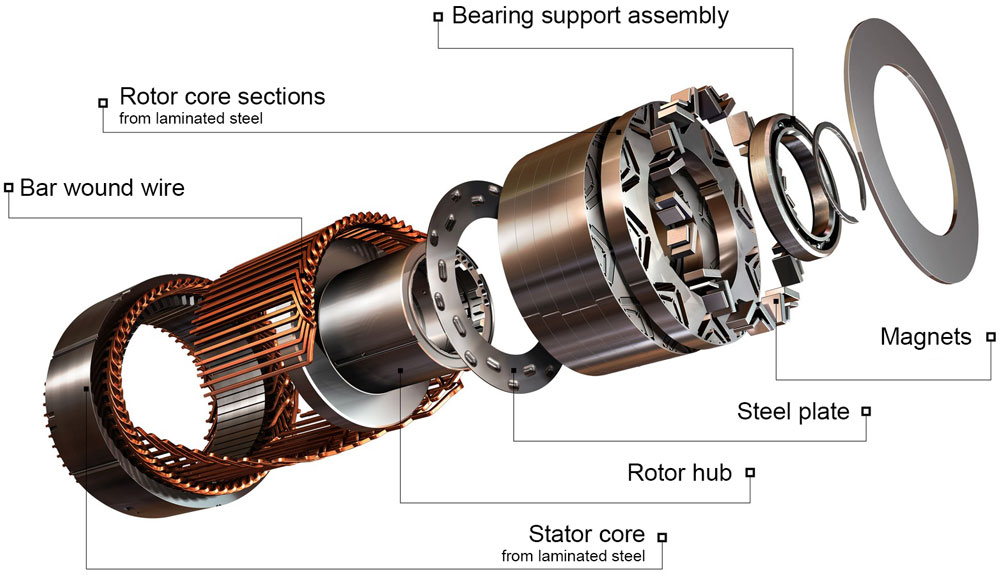
\includegraphics[width=0.7\textwidth]{sections/images/section1/ipmsm_disassembled_w1000.jpg}
    \caption{Working Components of \gls{pmsm}\cite{pmsm_review}}
    \label{fig:PMSM_figure}
\end{figure}
\subsection{Type of motor chosen}
There are different ways to design a \gls{pmsm}\cite{pmsm_review}, that won't be covered in this paper. For the sake of simplicity, in this project it has been decided to focus on a specific design configuration of electric motor, otherwise the dataset creation would become too complex, and much more experience would be needed in \gls{pmsm} design.

The two main part of an electric motor are the \emph{Stator} and the \emph{Rotor}, for both there are different design that could be chosen.

\textbf{DISCLAIMER}: Here i am assuming to use simplified notation, that could differ to precise keywords used in literature. This section is not a design review of electric motors, but just an help understanding some key design concept
\subsubsection{Rotor design chosen}
As it is the most simple \gls{pmsm} type to study and to deal with, \gls{spm} rotor has been chosen to create the dataset. The second motivation to this choice is that this design has been already covered by a previous university course here at MUNER\cite{MUNER}.

The characteristic of an \gls{spm} rotor is to have the magnets round shaped, and placed in the outer side of the rotor (as can be seen in \cref{fig:rotor_magnet_placement})

\begin{figure}[H]
    \centering
    \makebox[\textwidth][c]{
    %
    \begin{subfigure}{0.55\textwidth}
        \centering
        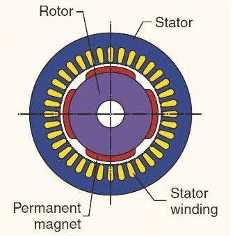
\includegraphics[width=.7\linewidth]{sections/images/section1/spm_example.jpg}
        \label{fig:spm_example}
        \caption{\glsxtrlong{spm}}
    \end{subfigure}
    %
    \begin{subfigure}{0.55\textwidth}
        \centering
        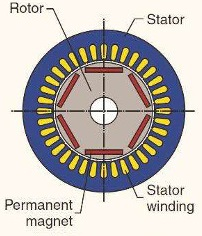
\includegraphics[width=.68\linewidth]{sections/images/section1/ipm_example.jpg}
        \caption{Interior Permanent Magnet}
        \label{fig:ipm_example}
    \end{subfigure}}
  \caption{Two of the most used rotor magnet placement}
  \label{fig:rotor_magnet_placement}
\end{figure}

\subsubsection{Winding layout chosen}
The decision of the stator design was easier due to the fewer option available.

The two main stator design (or better, winding layout) are \gls{dw} and \gls{fw}. There are advantages and disadvantages for both layouts, but \gls{fw} has been preferred for this project because demagnetization is more difficult to predict analytically. An example in \cref{fig:winding_placement}
\begin{figure}[H]
    \centering
    \makebox[\textwidth][c]{
    %
    \begin{subfigure}{0.55\textwidth}
        \centering
        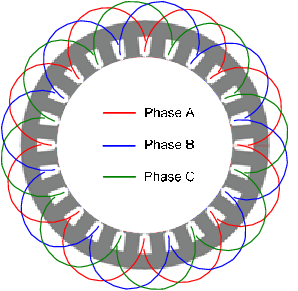
\includegraphics[width=.7\linewidth]{sections/images/section1/distribuited.png}
        \label{fig:dw_example}
        \caption{\glsxtrlong{dw}}
    \end{subfigure}
    %
    \begin{subfigure}{0.55\textwidth}
        \centering
        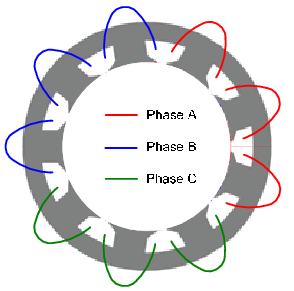
\includegraphics[width=.7\linewidth]{sections/images/section1/fractional.png}
        \caption{\glsxtrlong{fw}}
        \label{fig:fw_example}
    \end{subfigure}}
  \caption{Two of the most used rotor Winding layout}
  \label{fig:winding_placement}
\end{figure}

The wire inside the slots have been simplified as a normal round copper wire, without considering skin effects. Different copper inside slots can be seen in \cref{fig:copper_example}
\begin{figure}[H]
    \centering
    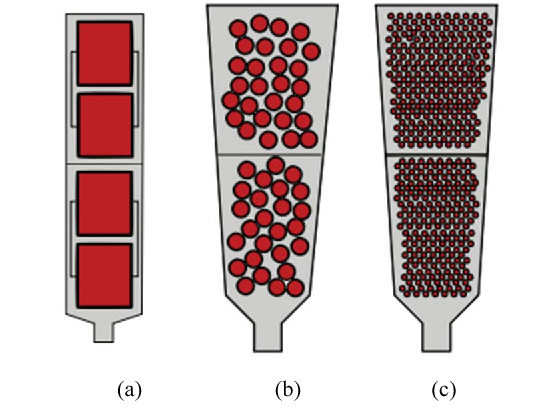
\includegraphics[width=0.5\textwidth]{sections/images/section1/copper_example.png}
    \caption{Slot area view: (a)hairpin, (b)round wire, (c)litz wire}
    \label{fig:copper_example}
\end{figure}
\subsection{Description of the problem}
Demagnetization of \gls{pmsm} motors is a tedious topic in high performance machines: It does happen due to high temperatures and high electric load during the utilization of the motor.

Demagnetization of a magnet happens if the magnetic field inside the magnet $H_{magn}$ is greater, in module, of its intrinsic coercivity $H_{CI}$(that depends on the material and the temperature of the magnet).

The analytical equation that describe when demagnetization happens is:
\begin{equation}\label{eq:demagn_formula_approx}
    |H_{magn}| = \left|\frac{\frac{N}{2}I-\frac{\delta_0}{\mu_0}B_r}{l_{magn}+\delta_0\frac{\mu_d}{\mu_0}}\right|<|H_{CI}|
\end{equation}
where
\begin{itemize}
    \item $N$: Series conductors per phase.
    \item $I$: Peak current crossing the windings.
    \item $\delta_0$: Airgap thickness.
    \item $\mu_0$: magnetic permeability of free space.
    \item $B_r=B_{r0}(1+\alpha_{B_{r}}(T-T_0))$: Magnet remanence.
    \item $l_{magn}$: magnet thickness.
    \item $\mu_d$: Permeability of the magnet.
    \item $H_{CI}=H_{CI0}(1+\alpha_{H_{CI}}(T-T_0))$: intrinsic coercivity
    \item $H_{CI0},B_{rI0}$: Reference Value.
    \item $\alpha_{H_{CI}}, \alpha_{B_{r}}$: temperature coefficient.
\end{itemize}

The downside of this equation, is that it assumes that the magnetic field produced by the magnet is sinusoidal, without taking in consideration side harmonics. 

\gls{fw} motors are known to produce an higher number of side harmonics, so this formula is not particularly suited for that stator type.

Another way to check demagnetization is to measure the $H_{magn}$ value inside magnets using \gls{fem} Software.

Temperature was set to the magnet temperature limit: $T=\SI{140}{\celsius}$ as datasheet. Magnet used is \emph{Cibas ren35h NeFeb}.
\subsection{Why this work could be useful?}
As already said, it is possible to check for demagnetization using using \gls{fem}, but that approach has different disadvantages:
\begin{itemize}
    \item The duration of \gls{fem} simulation can last up to tens of minutes $\rightarrow$ Design optimization time will be considerable.
    \item \gls{fem} simulation can only be used at the end ot the motor design process, when geometry has already been shaped $\rightarrow$ Precise prediction for demagnetization is not possible during early design stages.
\end{itemize}

This two disadvantages are particularly bad for high performance \gls{pmsm} motors used in automotive: those type of machines are usually pushed to the limit by exploiting their \gls{ol} capability.
\subsubsection{\texorpdfstring{\glsxtrlong{ol}}{Overload} of a motor}
The \gls{ol} is an important features of high performance electric motors: it is possible to inject more current, for a short interval of time time, and produce more torque than what the motor was built for.

How is it possible to run in \gls{ol} without damaging the motor? the electric/mechanic dynamics is relatively fast compared to the slow thermal dynamics: so to avoid overheating it is necessary to use \gls{ol} for a short period of time.

If the motor temperatures are kept in a safe range, the only concern about \gls{ol} is the demagnetization.
\subsubsection{\texorpdfstring{\glsxtrlong{ol}}{Overload} and Demagnetization}
As the approximated equation in \cref{eq:demagn_formula_approx} suggest, demagnetization can happen if the current $I$ is too high. This mean that for each motor it is possible to have a maximum overload current that it is not possible to exceed.
it can be useful to predict how much \gls{ol} it is possible to apply for two main reason:
\begin{itemize}
    \item Predict \gls{ol} at early development stage to modify it if different behavior are desired.
    \item Apply optimization algorithm at high speed.
\end{itemize}
\subsection{Proposed target of this work}
The target of this work is to create a machine learning tool capable to predict how much \gls{ol} is possible without going in demagnetization, given few initial parameters.

This work is made purely for didactic purpose, this is why a single type of motor is investigated, and limited parameters/materials can be chosen.


\section{Dataset Creation}
As already mentioned, the Dataset has been created with Matlab And FEMM. It was possible to create a script that simulates in \gls{fem} a randomly generated electric motor, and measure the magnetic field inside the magnets to check for demagnetization.

Thanks to Giacomo Sala, professor of Electric Motor Design at MUNER\cite{MUNER}, that provided to the students the code to easily simulate an electric motor using FEMM and Matlab.
\begin{figure}[H]
    \centering
    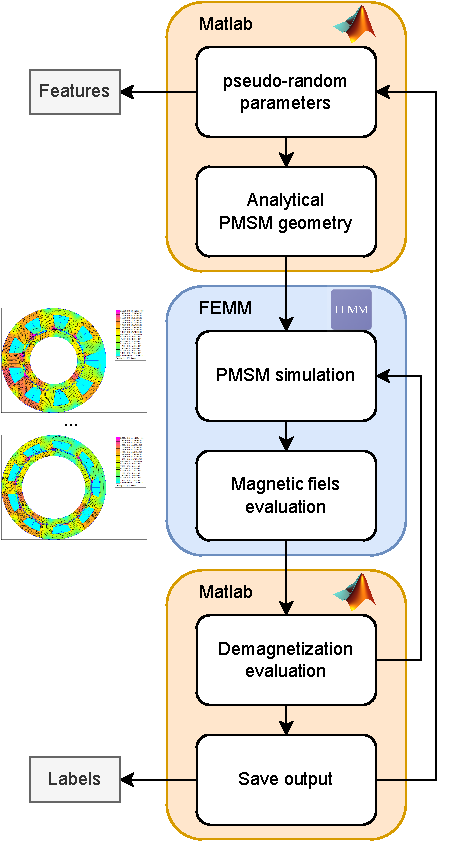
\includegraphics[width=0.54\textwidth]{sections/images/section2/dataset_creation.pdf}
    \caption{Dataset creation workflow}
    \label{fig:dataset_creation}
\end{figure}
The main steps of the dataset generation process are summarized in \cref{fig:dataset_creation}. In greater details the steps are:
\begin{enumerate}\label{tab:dataset_creation}
    \item Pseudo randomly generate the motor parameters and values, to be used as \emph{features}.
    \item Generate the motor geometry analytically.
    \item Run \gls{fem} simulation of the motor.
    \item Measure the magnetic field inside the magnets, and extrapolate the point where field is maximum.
    \item Compare the measured field to its maximum possible value $H_{CI}$.
    \item Repeat measurements until demagnetization happens.
    \item Save the last "safe" current overload value that will not create overload as a \emph{label}.
\end{enumerate}
\subsection{Features}
Features have been pseudo randomly generated: a known working motor configuration has been chosen, where some parameters (the features) have been changed randomly in a specific range.

It was not possible to chose the features completely randomly, or some motor configuration could have been physically impractical.

The features, and their range, are:
\begin{center}
    \begin{table}[H]
       \renewcommand{\arraystretch}{1.2}
        \centerline{
        \centering
        \begin{tabular}{|r|c|c|c|}
        \hline
        &Feature & Mean value & Range \\
        \hline
        $T_{spec}$&Nominal Torque&\SI{150}{\newton\metre}&$\pm$ \SI{75}{\newton\metre}\\
        \hline
        $W_{spec}$&Rated Speed&\SI{3.5}{\kilo\rpm}&$\pm$ \SI{1.75}{\kilo rpm}\\
        \hline
        $B{mr}$&Magnetic Loading&\SI{0.75}{\tesla}&$\pm$ \SI{0.375}{\tesla}\\
        \hline
        $\delta$&Electric Loading&\SI{4}{\kilo\ampere/\metre}&$\pm$ \SI{2}{\kilo\ampere/\metre}\\
        \hline
        $m$&Aspect Ratio&\SI{1.5}{}&$\pm$ \SI{0.75}{}\\
        \hline
        $S_o$&Slot Opening&\SI{5}{\milli\metre}&$\pm$ \SI{1.75}{\milli\metre}\\
        \hline
        $d_0$&Airgap Thikness&\SI{1.2}{\milli\metre}&$\pm$ \SI{0.42}{\milli\metre}\\
        \hline
        $l_{magn}$&Magnet height&$l_{magn0}$ from calculation&$l_{magn0}*1.5\pm l_{magn0}*0.1$\\
        \hline
        $h_4$&Slot Opening height&\SI{2}{\milli\metre}&$\pm$ \SI{0.7}{\milli\metre}\\
        \hline
        $h_3$&Wedge Height&\SI{5}{\milli\metre}&$\pm$ \SI{1.75}{\milli\metre}\\
        \hline
        \end{tabular}}
        \caption{Features summary}
    \end{table}
\end{center}
\subsubsection{Note on \texorpdfstring{$l_{magn}$}{Lmagn} }
The only feature that has not chosen like the others is the magnet height $l_{magn}$. This because $l_{magn}$ needs to be greater than a certain quantity (dependent on other chosen features), so it was not possible to randomize it from a given value. To make the output result of the simulations more interesting, it has been decided to increase the calculated value $l_{magn0}$ by $1.5$, and to randomize this last value: doing so, it was possible to see more variegate values of maximum overload in output.

If $l_{magn}$ was chosen only considering the initial calculation, we would have seen a lot of low overload value, and the labels would have been much less interesting.
\subsection{Labels}
Each simulation outputs a single label $OL_{max}$: a number which represents the maximum overload that the motor is capable before demagnetizing.
\subsubsection{Magnetic field \texorpdfstring{$H_{magn}$}{Hmagn} measurement}
The magnetic field is measured in \gls{fem} simulation along the perimeter of a circumference that touches the mean height of the magnet: an example can be seen as the red line in \cref{fig:measurment_line}
\begin{figure}[H]
    \centering
    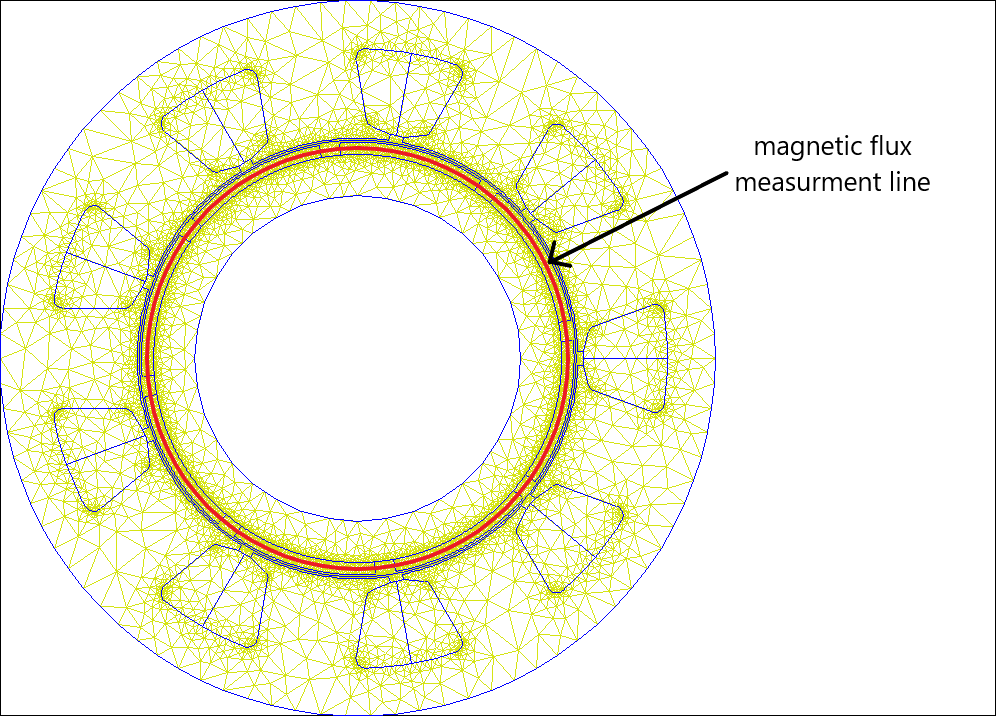
\includegraphics[width=0.6\textwidth]{sections/images/section2/measurment_line.png}
    \caption{Magnetic field measurement line example}
    \label{fig:measurment_line}
\end{figure}
\subsubsection{Maximum overload detection}
The overload detection and the labels output follows the following scheme:
\begin{enumerate}
    \item Matlab script starts by simulating the motor at nominal current.
    \item The maximum value of magnetic field along that line is find.
    \item Check if $|H_{magn}|<|H_{CI}|$.
    \item If the check is \textbf{true}: no demagnetization is happening, reiterate the simulation with increased current.
    \item If the check is \textbf{false}: demagnetization is happening, stop the simulation, save the last overload value as the label (that \gls{ol} will be the last one before demagnetization).
\end{enumerate}
This cycle is repeated for all the simulated motors.
\subsubsection{Note on label value}
Labels value are in a range between $0$ and $11$, where $0$ means no overload, and $11$ represents an overload of $6.5$.

To get the overload value $OL$ from the output of the script, the following equation needs to be applied:
\begin{equation}
    OL = \frac{Label}{2}+1
\end{equation}
\section{\texorpdfstring{\gls{ml}}{ML} Model}\label{sec:ML}
After the creation of the dataset, the main machine learning machine was trained and tested.

This remaining part has been developed on a Jupyter notebook, publicly available on Github and Kaggle alongside the dataset used.
\begin{itemize}
    \item Github repo: \url{https://github.com}
    \item Kaggle repo: \url{https://www.kaggle.com}
\end{itemize}
\subsection{Dataset analysis}
The dataset used has \texttt{7000} entries in total, each one representing a simulated motor.

Thanks to the various libraries used, it was possible to analyze data using intuitive graphical plots.
\subsubsection{Frequency plot}
\begin{figure}[H]
    \centering
    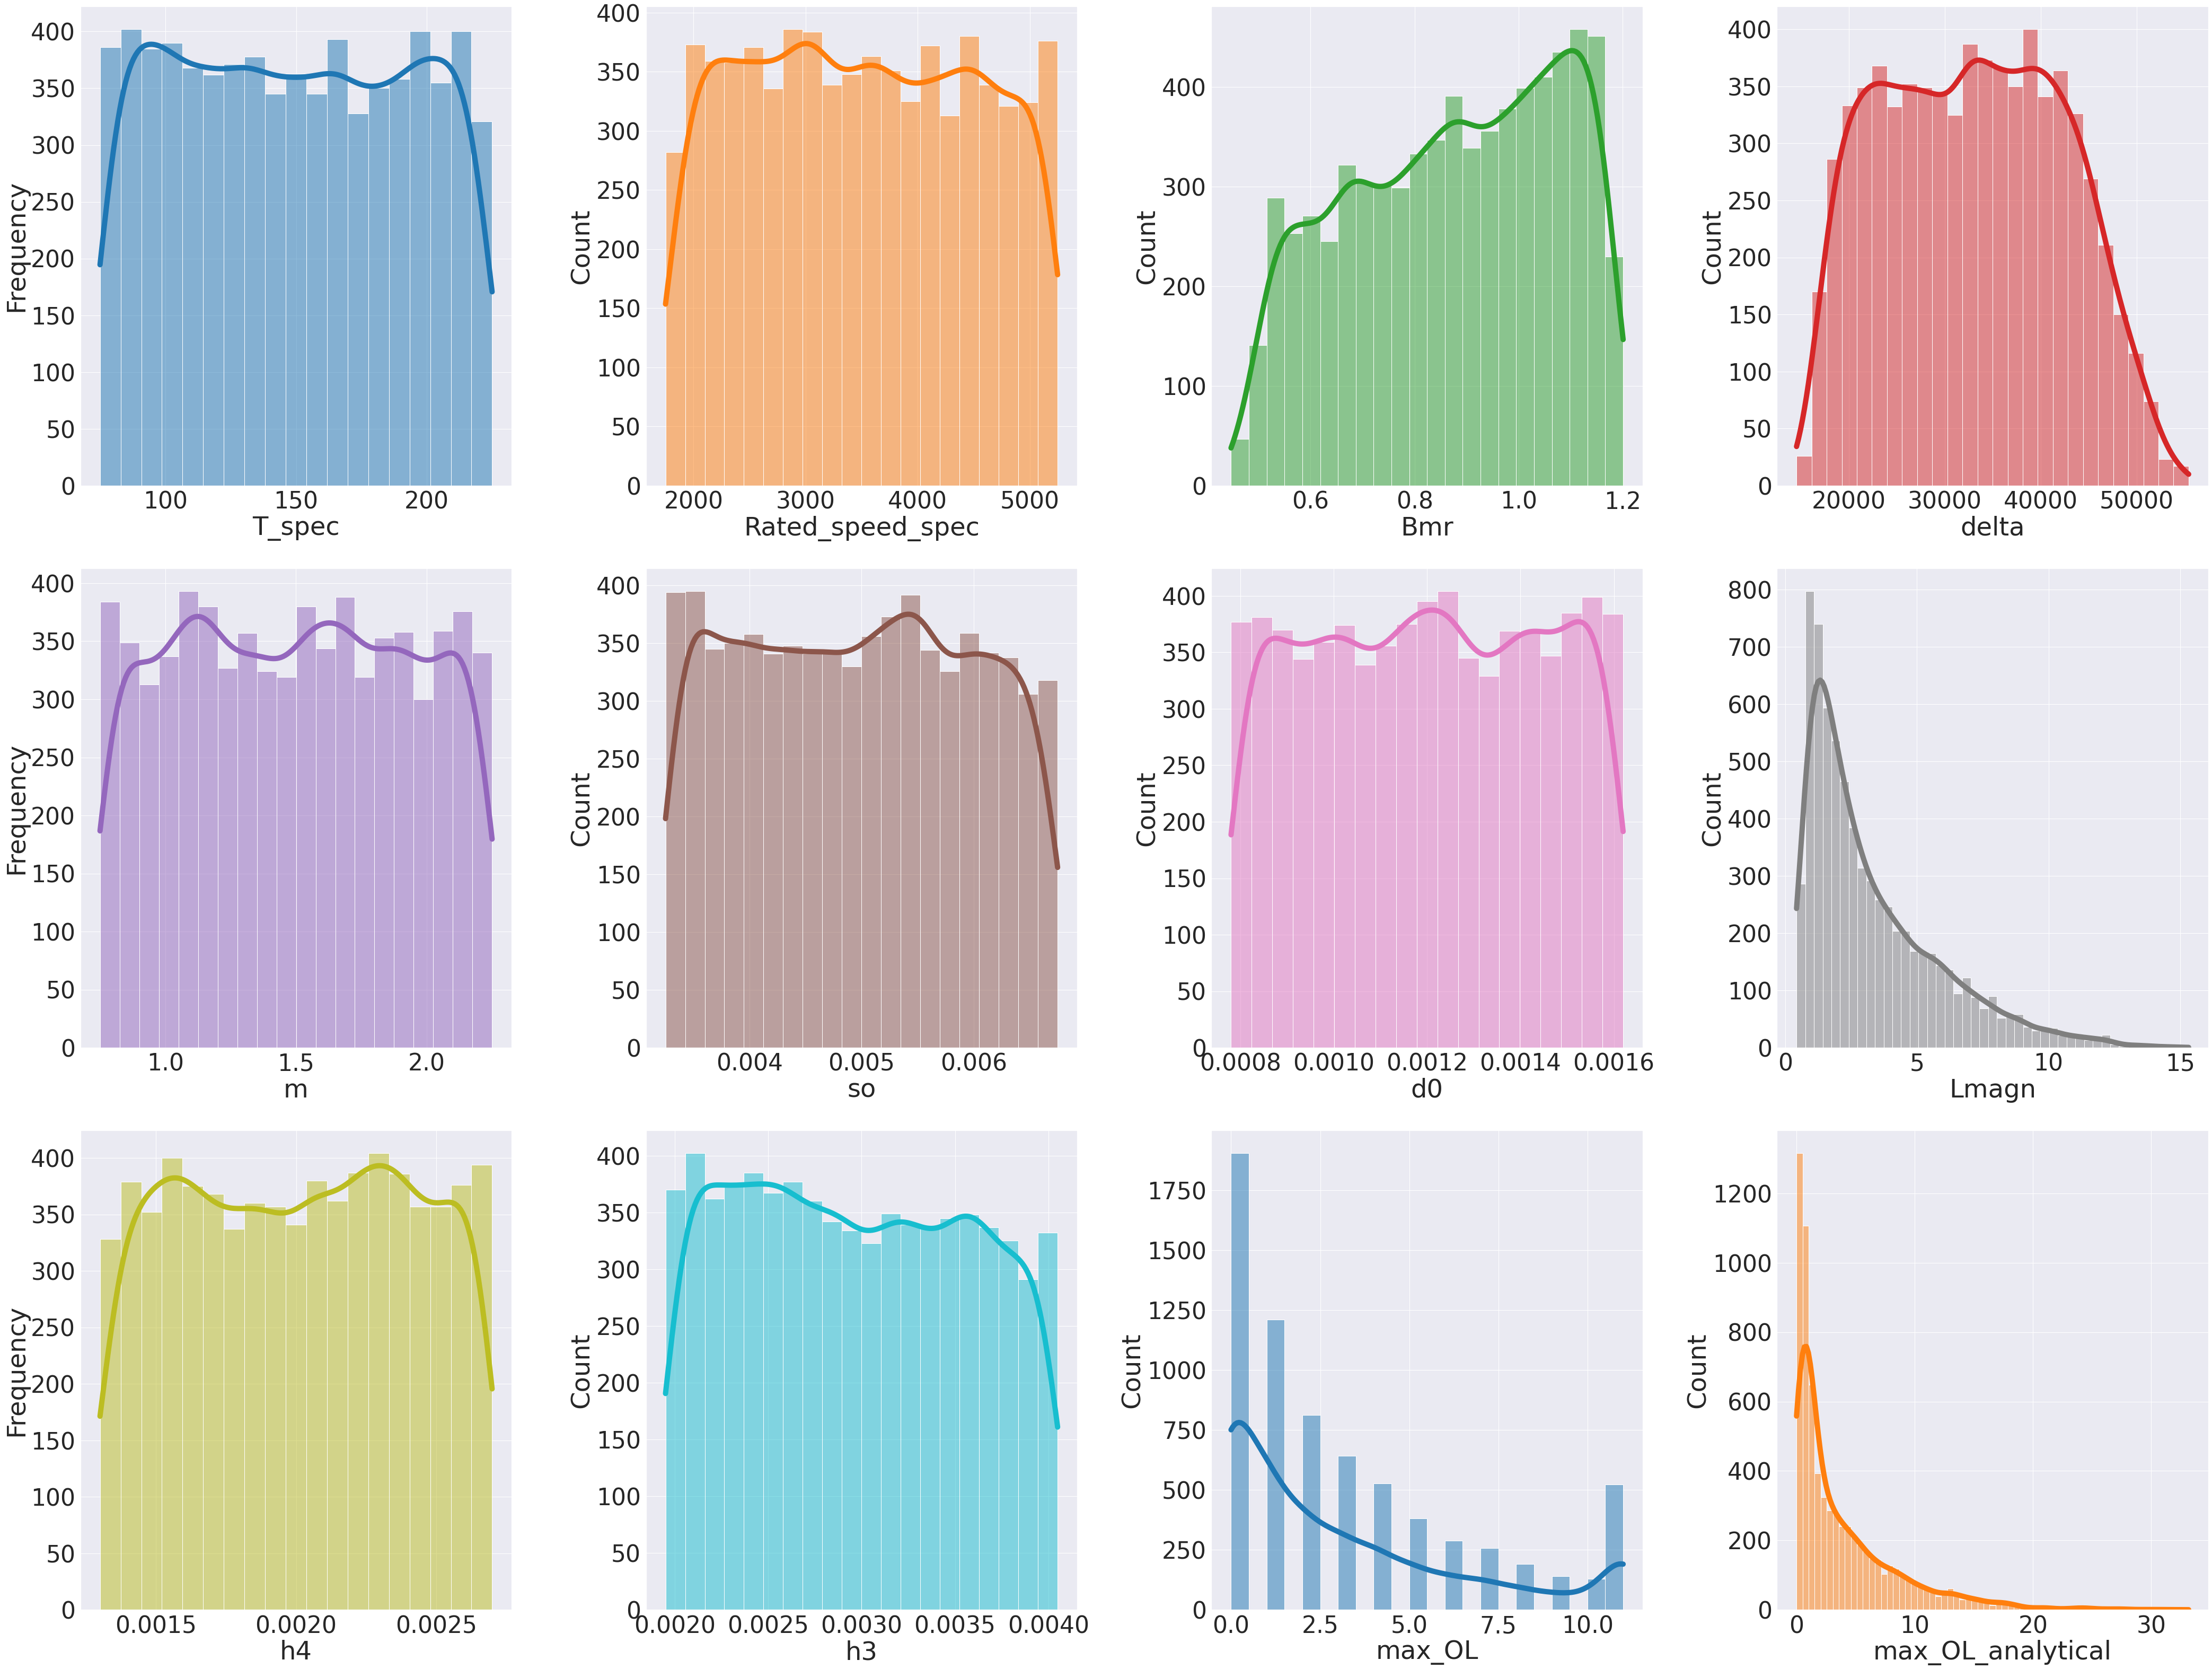
\includegraphics[width=0.6\textwidth]{sections/images/section3/frequency_plot.png}
    \caption{Frequency plot}
    \label{fig:freq_plot}
\end{figure}
The frequency plot in \cref{fig:freq_plot} shows that all the labels are randomly distributed, except fot the magnet height $L_{magn}$.

The last two plots, shows the distribution of \gls{fem} and analytical prediction.
\subsubsection{Correlation Matrix}
\begin{figure}[H]
    \centering
    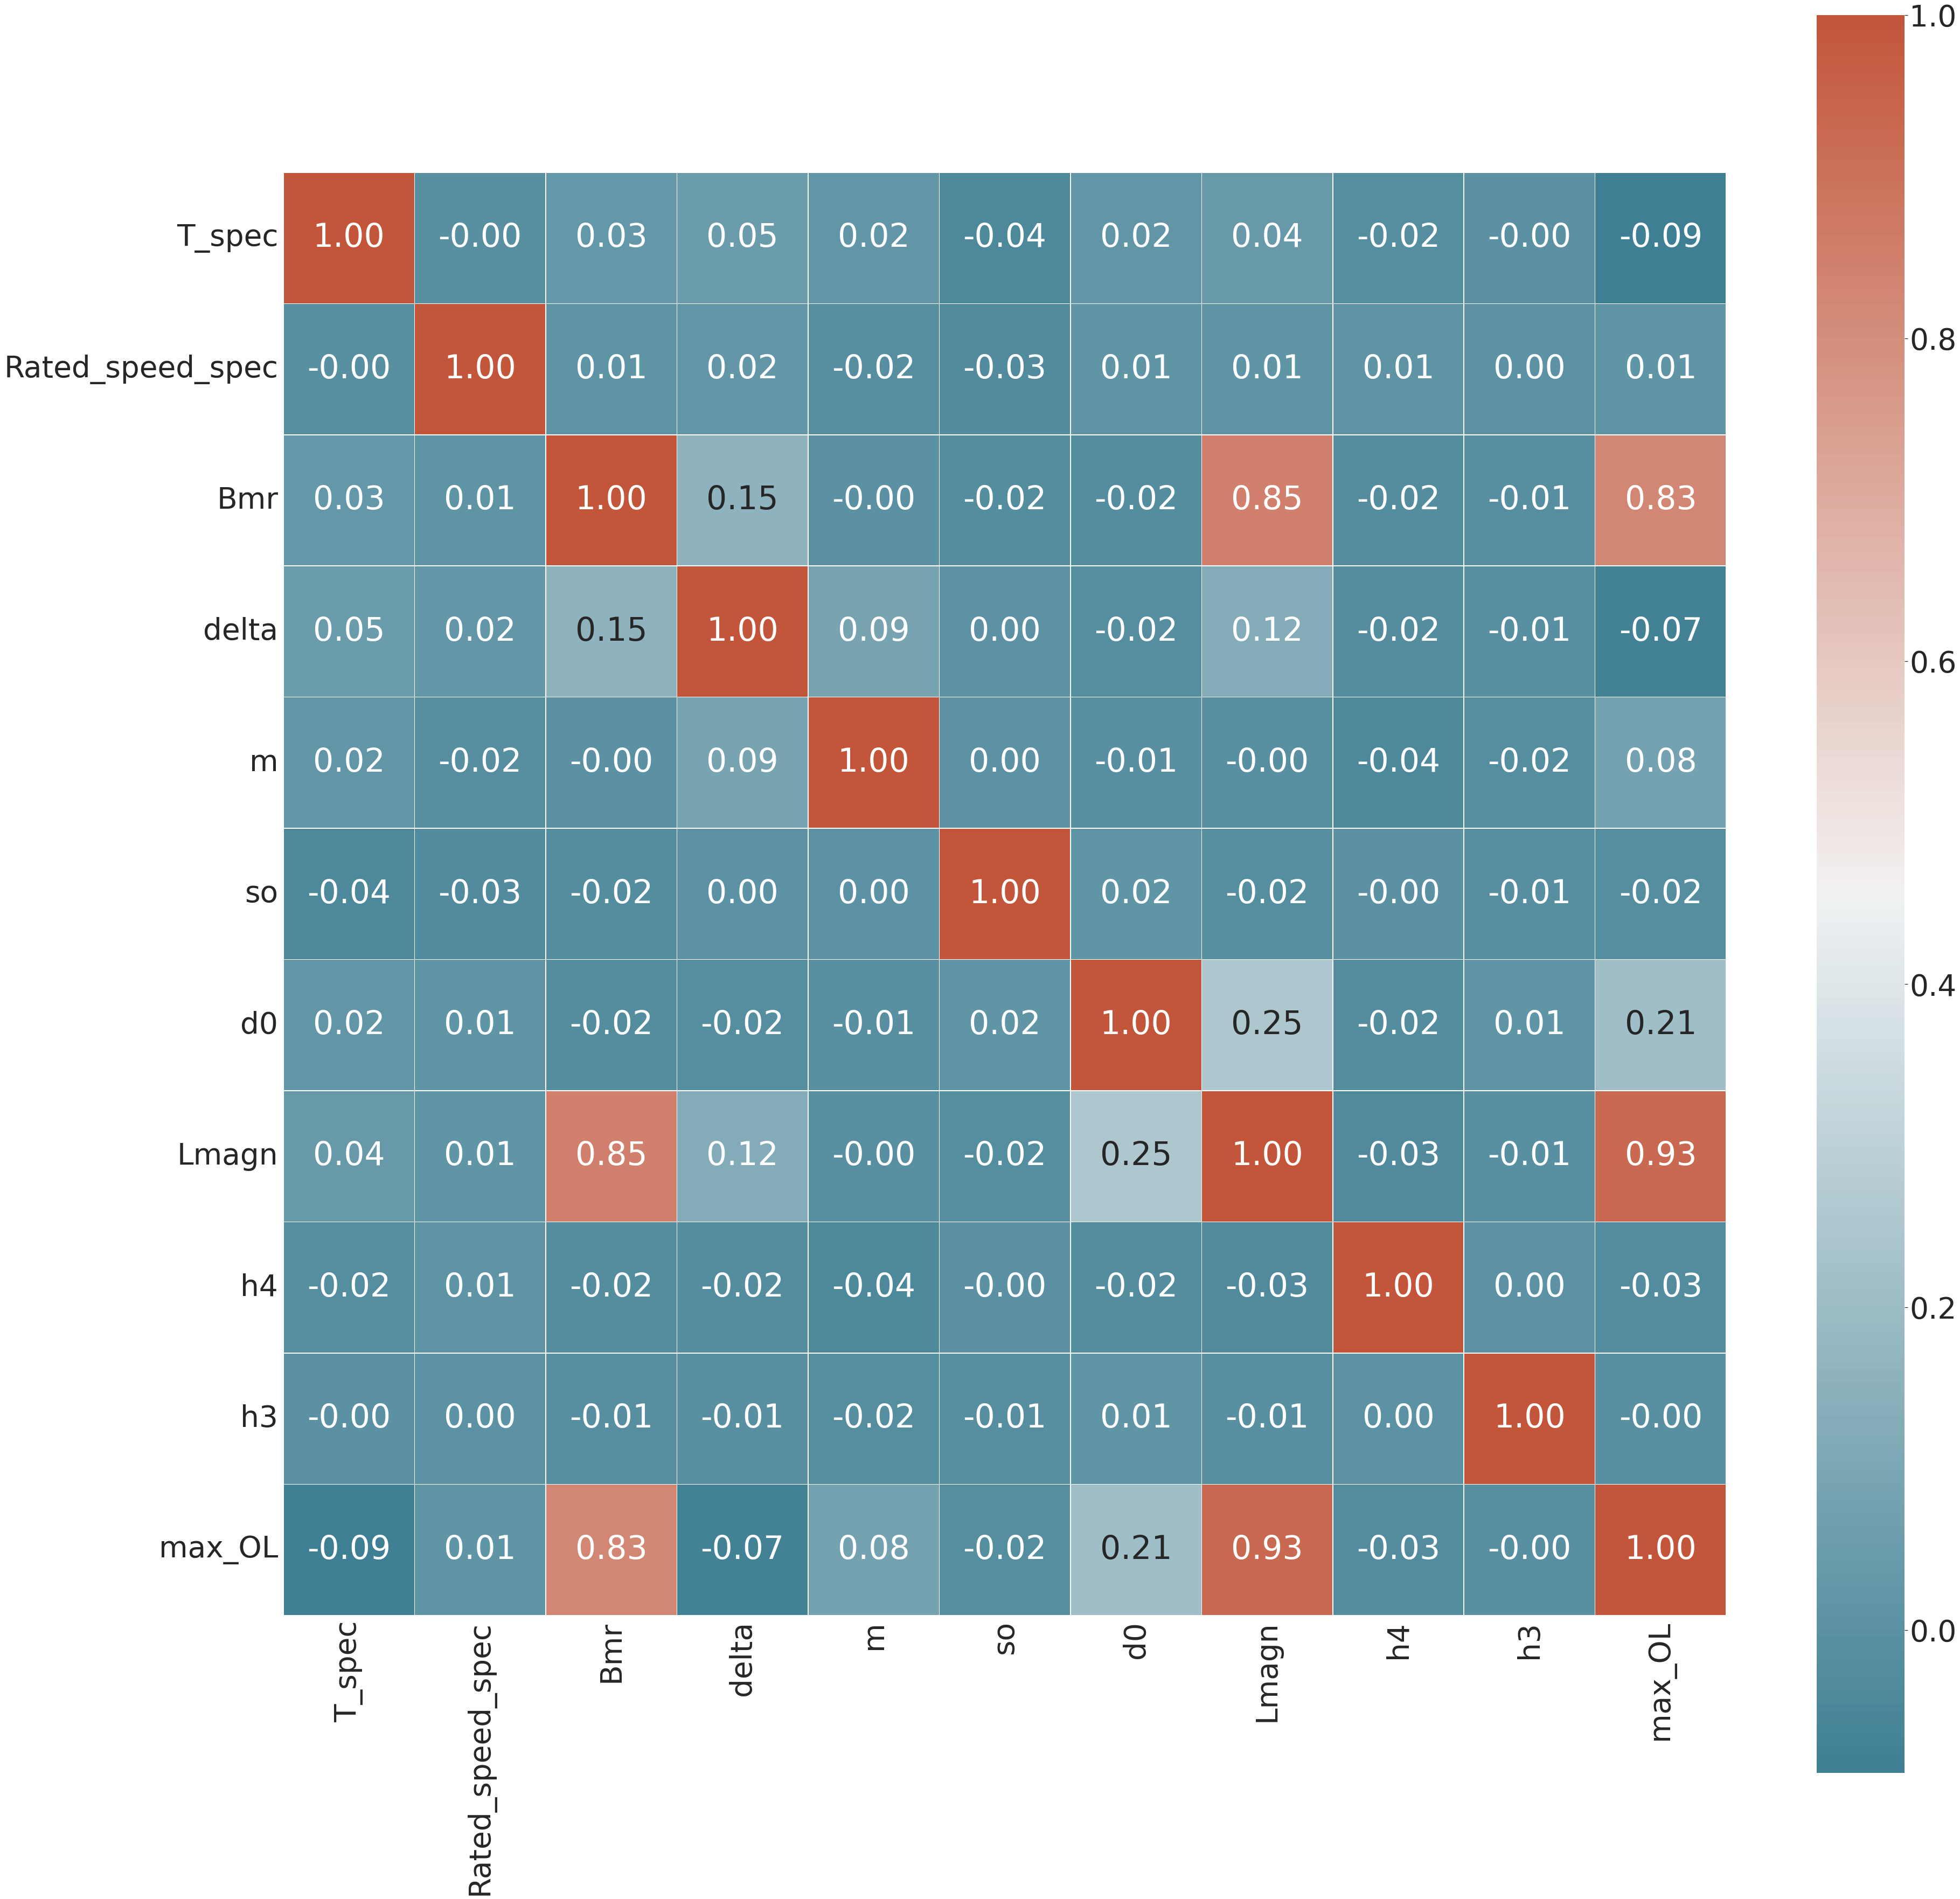
\includegraphics[width=0.6\textwidth]{sections/images/section3/correlation_matrix.png}
    \caption{Correlation Matrix}
    \label{fig:corr_matrix}
\end{figure}
As it is possible to see from the correlation matrix in \cref{fig:corr_matrix}, the magnet height $L_{magn}$ and the magnetic loading $B_{mr}$ are highly correlated with the maximum overload.
\subsubsection{Dataset Split}
The dataset was split in three different set: 
\begin{itemize}
    \item Train set: used to train the Machine.
    \item Test set: Used for the final evaluation of the Machine.
    \item Validation set: used to validate the Machine during the training.
\end{itemize}
\subsubsection{Stratification}
Stratification is used to be sure that the proportion of labels in the sample produced will be the same as the proportion of labels in the dataset. This will increase the reproducibility.
\subsection{Metrics}
There are different metrics useful to identify a good model.

Those metrics have been introduced for binary classification, but it is possible to extend those to multi class.
Notation:
\begin{itemize}
    \item $TP$: True Positive.
    \item $TN$: True Negative.
    \item $FP$: False Positive.
    \item $FN$: False Negative.
\end{itemize}
\subsubsection{Precision}
Number of items correctly identified as positive out of the total items identified as positive:
\begin{equation}
    \frac{TP}{TP+FP}
\end{equation}
\subsubsection{Recall}
Number of items correctly identified as positive out of the total actual positives:
\begin{equation}
    \frac{TP}{TP+FN}
\end{equation}
\subsubsection{Accuracy}
Number of items correctly identified as either truly positive or truly negative out of the total number of items:
\begin{equation}
    \frac{TP+TN}{TP+TN+FP+FN}
\end{equation}
Usually it is the most used metrics for a first evaluation of the model.
\subsubsection{F1-Score}
The harmonic average of the precision and recall, it measures the effectiveness of identification when just as much importance is given to recall as to precision:
\begin{equation}
    \frac{TP+TN}{TP+TN+FP+FN}
\end{equation}
In multiclass, it can be calculated as an average of all the F1 score, or as a weighted average. Weights can be the number of samples for each category.
\subsubsection{Loss}
Loss is a number indicating how bad the model's prediction was on a single example. It is very important because it is the number that a model should seek to minimize during training.

Usually \gls{mse} is used as the loss function for regression:
\begin{equation}
    MSE=\frac{1}{N}\sum_{(x,y)\in D}\left(y-Prediction(x)\right)^2
\end{equation}
In multiclass classification, categorical Crossentropy is the most used:
\begin{equation}
    CrossEntropyLoss=-(y_i\log(\hat{y}_i)+(1-y_i)\log(1-\hat{y}_i))
\end{equation}
\subsection{Regression model}
The first machine trained is a linear regression model, that uses one or multiple parameters. The decision to use such simple machine is to start by using something simple and understandable, and it is interesting to see how performance increases by introducing complexity on the machine.
\subsubsection{Linear regression - one variable}
In order to train such machine with one variable, we need to chose a suitable feature that is going to weight a lot on the output label. In \cref{fig:corr_matrix} it is possible to see that $L_{magn}$ is the most correlated to the label, so that feature has chosen.
The trained model can be summarized as follows:
\begin{lstlisting}[basicstyle=\ttfamily\footnotesize]
Model: "sequential"
_________________________________________________________________
    Layer (type)                Output Shape              Param #   
=================================================================
    flatten (Flatten)           (None, 1)                 0         
                                                                    
    dense (Dense)               (None, 1)                 2         
                                                                    
=================================================================
Total params: 2
Trainable params: 2
Non-trainable params: 0
_________________________________________________________________
\end{lstlisting}
Information about the training:
\begin{center}
    \begin{table}[H]
       \renewcommand{\arraystretch}{1.2}
        \centerline{
        \centering
        \begin{tabular}{|r|c|c|c|}
        \hline
        Optimizer &epoch & loss  & metrics \\
        \hline
        Adam & $150$ & mean\_absolute\_error&accuracy\\
        \hline
        \end{tabular}}
    \end{table}
\end{center}
The result of this machine can be visualized in \cref{fig:linear_one_veariable}, and its result metrics are:
\begin{center}
    \begin{table}[H]
       \renewcommand{\arraystretch}{1.2}
        \centerline{
        \centering
        \begin{tabular}{|c|c|}
        \hline
        Validation loss &Validation accuracy \\
        \hline
        $0.8425$ & $0.3482$ \\
        \hline
        \end{tabular}}
    \end{table}
\end{center}
\begin{figure}[H]
    \centering
    \makebox[\textwidth][c]{
    %
    \begin{subfigure}{0.55\textwidth}
        \centering
        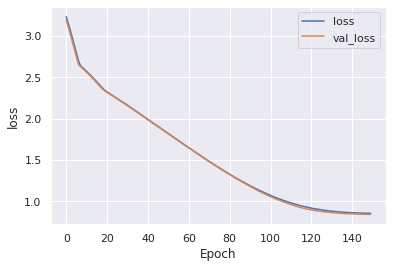
\includegraphics[width=.9\linewidth]{sections/images/section3/linear_one_veariable_loss.png}
        \caption{loss}
    \end{subfigure}
    %
    \begin{subfigure}{0.55\textwidth}
        \centering
        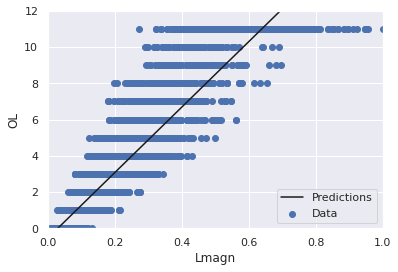
\includegraphics[width=.9\linewidth]{sections/images/section3/linear_one_veariable_plot.png}
        \caption{plot}
    \end{subfigure}}
  \caption{Linear regression - one variable}
  \label{fig:linear_one_veariable}
\end{figure}
%%%%%%%%%%%%%%%%%%%%%%%%%%%%%%%%%%%%%%%%%%%%%%%%%%%%%%%%%%%%%%%%%%%%%%%%%%%
\subsubsection{Linear regression - multi variable}
Now the linear regression machine have all the features in input, so we except to have better metrics.
The trained model can be summarized as follows:
\begin{lstlisting}[basicstyle=\ttfamily\footnotesize]
Model: "sequential"
_________________________________________________________________
    Layer (type)                Output Shape              Param #   
=================================================================
    flatten (Flatten)           (None, 10)                0         
                                                                    
    dense (Dense)               (None, 1)                 11        
                                                                    
=================================================================
Total params: 11
Trainable params: 11
Non-trainable params: 0
_________________________________________________________________
\end{lstlisting}
Information about the training:
\begin{center}
    \begin{table}[H]
       \renewcommand{\arraystretch}{1.2}
        \centerline{
        \centering
        \begin{tabular}{|r|c|c|c|}
        \hline
        Optimizer &epoch & loss  & metrics \\
        \hline
        Adam & $150$ & mean\_absolute\_error&accuracy\\
        \hline
        \end{tabular}}
    \end{table}
\end{center}
The result of this machine can be visualized in \cref{fig:linear_multi_veariable}, and its result metrics are:
\begin{center}
    \begin{table}[H]
       \renewcommand{\arraystretch}{1.2}
        \centerline{
        \centering
        \begin{tabular}{|c|c|}
        \hline
        Validation loss &Validation accuracy \\
        \hline
        $0.6756$ & $0.4089$ \\
        \hline
        \end{tabular}}
    \end{table}
\end{center}
\begin{figure}[H]
    \centering
    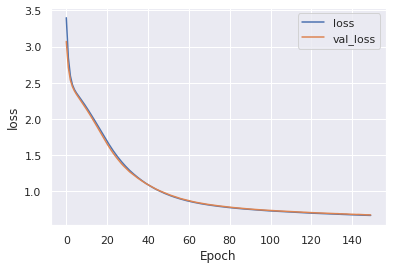
\includegraphics[width=.5\linewidth]{sections/images/section3/linear_multi_veariable.png}
    \caption{Linear regression - one variable - loss}
    \label{fig:linear_multi_veariable}
\end{figure}
%%%%%%%%%%%%%%%%%%%%%%%%%%%%%%%%%%%%%%%%%%%%%%%%%%%%%%%%%%%%%%%%%%
\subsubsection{NON Linear regression - one variable \texorpdfstring{$L_{magn}$}{Lmagn}}
$L_{magn}$ is again the feature used to train this one variable regression, but now a non linear regression will be used.
A \gls{dnn} has been used to create this non linear regression machine.
The trained model can be summarized as follows:
\begin{lstlisting}[basicstyle=\ttfamily\footnotesize]
Model: "sequential"
_________________________________________________________________
    Layer (type)                Output Shape              Param #   
=================================================================
    flatten (Flatten)           (None, 1)                 0         
                                                                    
    dense (Dense)               (None, 32)                64        
                                                                    
    dense_1 (Dense)             (None, 64)                2112      
                                                                    
    dense_2 (Dense)             (None, 128)               8320      
                                                                    
    dense_3 (Dense)             (None, 1)                 129       
                                                                    
=================================================================
Total params: 10,625
Trainable params: 10,625
Non-trainable params: 0
_________________________________________________________________
\end{lstlisting}
Information about the training:
\begin{center}
    \begin{table}[H]
       \renewcommand{\arraystretch}{1.2}
        \centerline{
        \centering
        \begin{tabular}{|r|c|c|c|}
        \hline
        Optimizer &epoch & loss  & metrics \\
        \hline
        Adam & $150$ & mean\_absolute\_error&accuracy\\
        \hline
        \end{tabular}}
    \end{table}
\end{center}
The result of this machine can be visualized in \cref{fig:non_linear_one_veariable}, and its result metrics are:
\begin{center}
    \begin{table}[H]
       \renewcommand{\arraystretch}{1.2}
        \centerline{
        \centering
        \begin{tabular}{|c|c|}
        \hline
        Validation loss &Validation accuracy \\
        \hline
        $0.7681$ & $0.3518$ \\
        \hline
        \end{tabular}}
    \end{table}
\end{center}
\begin{figure}[H]
    \centering
    \makebox[\textwidth][c]{
    %
    \begin{subfigure}{0.55\textwidth}
        \centering
        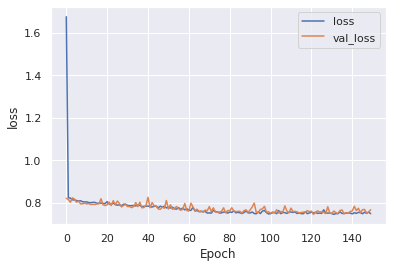
\includegraphics[width=.9\linewidth]{sections/images/section3/non_linear_one_veariable_loss.png}
        \caption{loss}
    \end{subfigure}
    %
    \begin{subfigure}{0.55\textwidth}
        \centering
        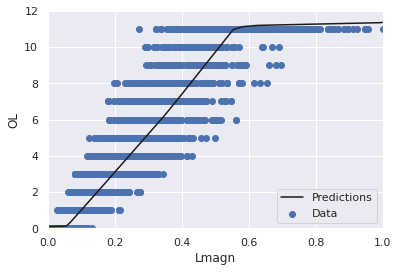
\includegraphics[width=.9\linewidth]{sections/images/section3/non_linear_one_veariable_plot.png}
        \caption{plot}
    \end{subfigure}}
  \caption{NON Linear regression - one variable - $L_{magn}$}
  \label{fig:non_linear_one_veariable}
\end{figure}
%%%%%%%%%%%%%%%%%%%%%%%%%%%%%%%%%%%%%%%%%%%%%%%%%%%%%%%%%%%%%%%%%%
\subsubsection{NON Linear regression - one variable \texorpdfstring{$B_{mr}$}{Bmr}}
The \gls{dnn} non linear regression machine is the sames before, but now the feature used is $B_{mr}$: the second most relevant according to the correlation matrix (\cref{fig:corr_matrix}).
The trained model can be summarized as follows:
\begin{lstlisting}[basicstyle=\ttfamily\footnotesize]
Model: "sequential"
_________________________________________________________________
    Layer (type)                Output Shape              Param #   
=================================================================
    flatten (Flatten)           (None, 1)                 0         
                                                                    
    dense (Dense)               (None, 32)                64        
                                                                    
    dense_1 (Dense)             (None, 64)                2112      
                                                                    
    dense_2 (Dense)             (None, 128)               8320      
                                                                    
    dense_3 (Dense)             (None, 1)                 129       
                                                                    
=================================================================
Total params: 10,625
Trainable params: 10,625
Non-trainable params: 0
_________________________________________________________________
\end{lstlisting}
Information about the training:
\begin{center}
    \begin{table}[H]
       \renewcommand{\arraystretch}{1.2}
        \centerline{
        \centering
        \begin{tabular}{|r|c|c|c|}
        \hline
        Optimizer &epoch & loss  & metrics \\
        \hline
        Adam & $150$ & mean\_absolute\_error&accuracy\\
        \hline
        \end{tabular}}
    \end{table}
\end{center}
The result of this machine can be visualized in \cref{fig:non_linear_one_bmr_veariable}, and its result metrics are:
\begin{center}
    \begin{table}[H]
       \renewcommand{\arraystretch}{1.2}
        \centerline{
        \centering
        \begin{tabular}{|c|c|}
        \hline
        Validation loss &Validation accuracy \\
        \hline
        $1.0235$ & $0.3357$ \\
        \hline
        \end{tabular}}
    \end{table}
\end{center}
\begin{figure}[H]
    \centering
    \makebox[\textwidth][c]{
    %
    \begin{subfigure}{0.55\textwidth}
        \centering
        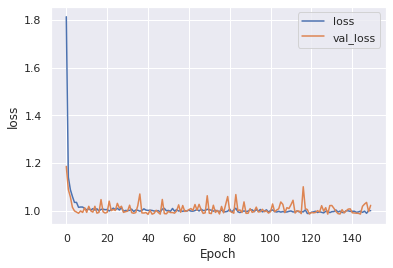
\includegraphics[width=.9\linewidth]{sections/images/section3/non_linear_one_veariable_bmr_loss.png}
        \caption{loss}
    \end{subfigure}
    %
    \begin{subfigure}{0.55\textwidth}
        \centering
        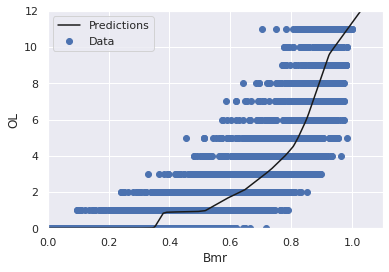
\includegraphics[width=.9\linewidth]{sections/images/section3/non_linear_one_veariable_bmr_plot.png}
        \caption{plot}
    \end{subfigure}}
  \caption{NON Linear regression - one variable - $B_{mr}$}
  \label{fig:non_linear_one_bmr_veariable}
\end{figure}
%%%%%%%%%%%%%%%%%%%%%%%%%%%%%%%%%%%%%%%%%%%%%%%%%%%%%%%%%%%%%%%%%%%%%%%%%%%
\subsubsection{NON Linear regression - multi variable}
Now the non linear regression machine utilize in input all the features, so we except to have better metrics. The depth of the network is increased to try reaching an useful value of metrics. The trained model can be summarized as follows:
\begin{lstlisting}[basicstyle=\ttfamily\footnotesize]
Model: "sequential"
_________________________________________________________________
    Layer (type)                Output Shape              Param #   
=================================================================
    flatten (Flatten)           (None, 10)                0         
                                                                    
    dense (Dense)               (None, 32)                352       
                                                                    
    dense_1 (Dense)             (None, 64)                2112      
                                                                    
    dense_2 (Dense)             (None, 128)               8320      
                                                                    
    dense_3 (Dense)             (None, 256)               33024     
                                                                    
    dense_4 (Dense)             (None, 1)                 257       
                                                                    
=================================================================
Total params: 44,065
Trainable params: 44,065
Non-trainable params: 0
_________________________________________________________________
\end{lstlisting}
Information about the training:
\begin{center}
    \begin{table}[H]
       \renewcommand{\arraystretch}{1.2}
        \centerline{
        \centering
        \begin{tabular}{|r|c|c|c|}
        \hline
        Optimizer &epoch & loss  & metrics \\
        \hline
        Adam & $150$ & mean\_absolute\_error&accuracy\\
        \hline
        \end{tabular}}
    \end{table}
\end{center}
The result of this machine can be visualized in \cref{fig:non_linear_multi_veariable}, and its result metrics are:
\begin{center}
    \begin{table}[H]
       \renewcommand{\arraystretch}{1.2}
        \centerline{
        \centering
        \begin{tabular}{|c|c|}
        \hline
        Validation loss &Validation accuracy \\
        \hline
        $0.1590$ & $0.4339$ \\
        \hline
        \end{tabular}}
    \end{table}
\end{center}
\begin{figure}[H]
    \centering
    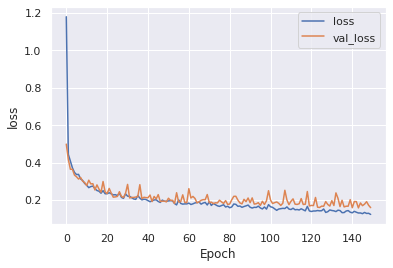
\includegraphics[width=.5\linewidth]{sections/images/section3/non_linear_multi_veariable_loss.png}
    \caption{non Linear regression - Multi variable - loss}
    \label{fig:non_linear_multi_veariable}
\end{figure}
Accuracy and loss are the highest until now, but are still unusable in real word applications.
%%%%%%%%%%%%%%%%%%%%%%%%%%%%%%%%%%%%%%%%%%%%%%%%%%%%%%%%%%%%%%%%%%%%%%%%%%%
\subsection{Classification \texorpdfstring{\glsxtrlong{dnn}}{Deep Neural Network}}
The machine using classification gives the best result for our problem, as it will be seen trough the metrics. The trained \gls{dnn} model has been chosen by a trial and error approach, and it is quite deep. The trained model can be summarized as follows:
\begin{lstlisting}[basicstyle=\ttfamily\footnotesize]
Model: "sequential"
_________________________________________________________________
    Layer (type)                Output Shape              Param #   
=================================================================
    flatten (Flatten)           (None, 10)                0         
                                                                    
    dense (Dense)               (None, 32)                352       
                                                                    
    dense_1 (Dense)             (None, 64)                2112      
                                                                    
    dense_2 (Dense)             (None, 128)               8320      
                                                                    
    dense_3 (Dense)             (None, 256)               33024     
                                                                    
    dense_4 (Dense)             (None, 12)                3084      
                                                                    
=================================================================
Total params: 46,892
Trainable params: 46,892
Non-trainable params: 0
_________________________________________________________________
\end{lstlisting}
Information about the training:
\begin{center}
    \begin{table}[H]
       \renewcommand{\arraystretch}{1.2}
        \centerline{
        \centering
        \begin{tabular}{|r|c|c|c|}
        \hline
        Optimizer &epoch & loss  & metrics \\
        \hline
        Adam & $150$ & SparseCategoricalCrossentropy&accuracy\\
        \hline
        \end{tabular}}
    \end{table}
\end{center}
The result of this machine can be visualized in \cref{fig:DNN_classification}, and its result metrics are:
\begin{center}
    \begin{table}[H]
       \renewcommand{\arraystretch}{1.2}
        \centerline{
        \centering
        \begin{tabular}{|c|c|}
        \hline
        Validation loss &Validation accuracy \\
        \hline
        $0.2841$ & $0.8893$ \\
        \hline
        \end{tabular}}
    \end{table}
\end{center}
\begin{figure}[H]
    \centering
    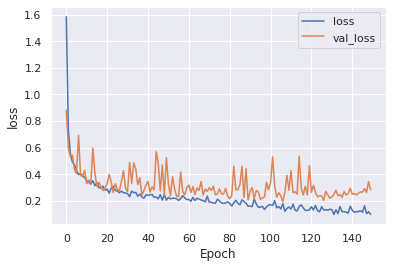
\includegraphics[width=.5\linewidth]{sections/images/section3/DNN_classification.png}
    \caption{\gls{dnn} Classification - loss}
    \label{fig:DNN_classification}
\end{figure}
\subsubsection{Evaluation with Test data}
It is assumed that it is the most performing network for our model, so it is suitable to evaluate it using the test data. The result metrics of the \gls{dnn} classification model are:
\begin{center}
    \begin{table}[H]
       \renewcommand{\arraystretch}{1.2}
        \centerline{
        \centering
        \begin{tabular}{|c|c|}
        \hline
        Validation loss &Validation accuracy \\
        \hline
        $0.2963$ & $0.9029$ \\
        \hline
        \end{tabular}}
    \end{table}
\end{center}
It can be seen that Loss increases compared with the non linear regression - multi variable. This is excepted because regression take in consideration the distance between output and labels more than a classification, and our problem is more prone to regression by design.

\textbf{NOTE:} comparing two losses, having different loss functions (like in this case) is not completely correct. Accuracy should be used instead.

Other metrics can be obtained, like the Precision, Recall and f1-score:
\begin{lstlisting}[basicstyle=\ttfamily\footnotesize]
              precision    recall  f1-score   support
       
           0      0.979     0.987     0.983       381
           1      0.950     0.938     0.944       242
           2      0.929     0.883     0.905       162
           3      0.836     0.953     0.891       128
           4      0.812     0.867     0.839       105
           5      0.789     0.737     0.762        76
           6      0.811     0.741     0.775        58
           7      0.766     0.706     0.735        51
           8      0.737     0.737     0.737        38
           9      0.793     0.821     0.807        28
          10      0.724     0.808     0.764        26
          11      1.000     0.933     0.966       105

    accuracy                          0.903      1400
   macro avg      0.844     0.843     0.842      1400
weighted avg      0.904     0.903     0.903      1400
\end{lstlisting}
Another interesting plot to see is the confusion matrix in \cref{fig:confusion_matrix}. It can give an intuitive idea on the precision and loss of the network by using colors.
\begin{figure}[H]
    \centering
    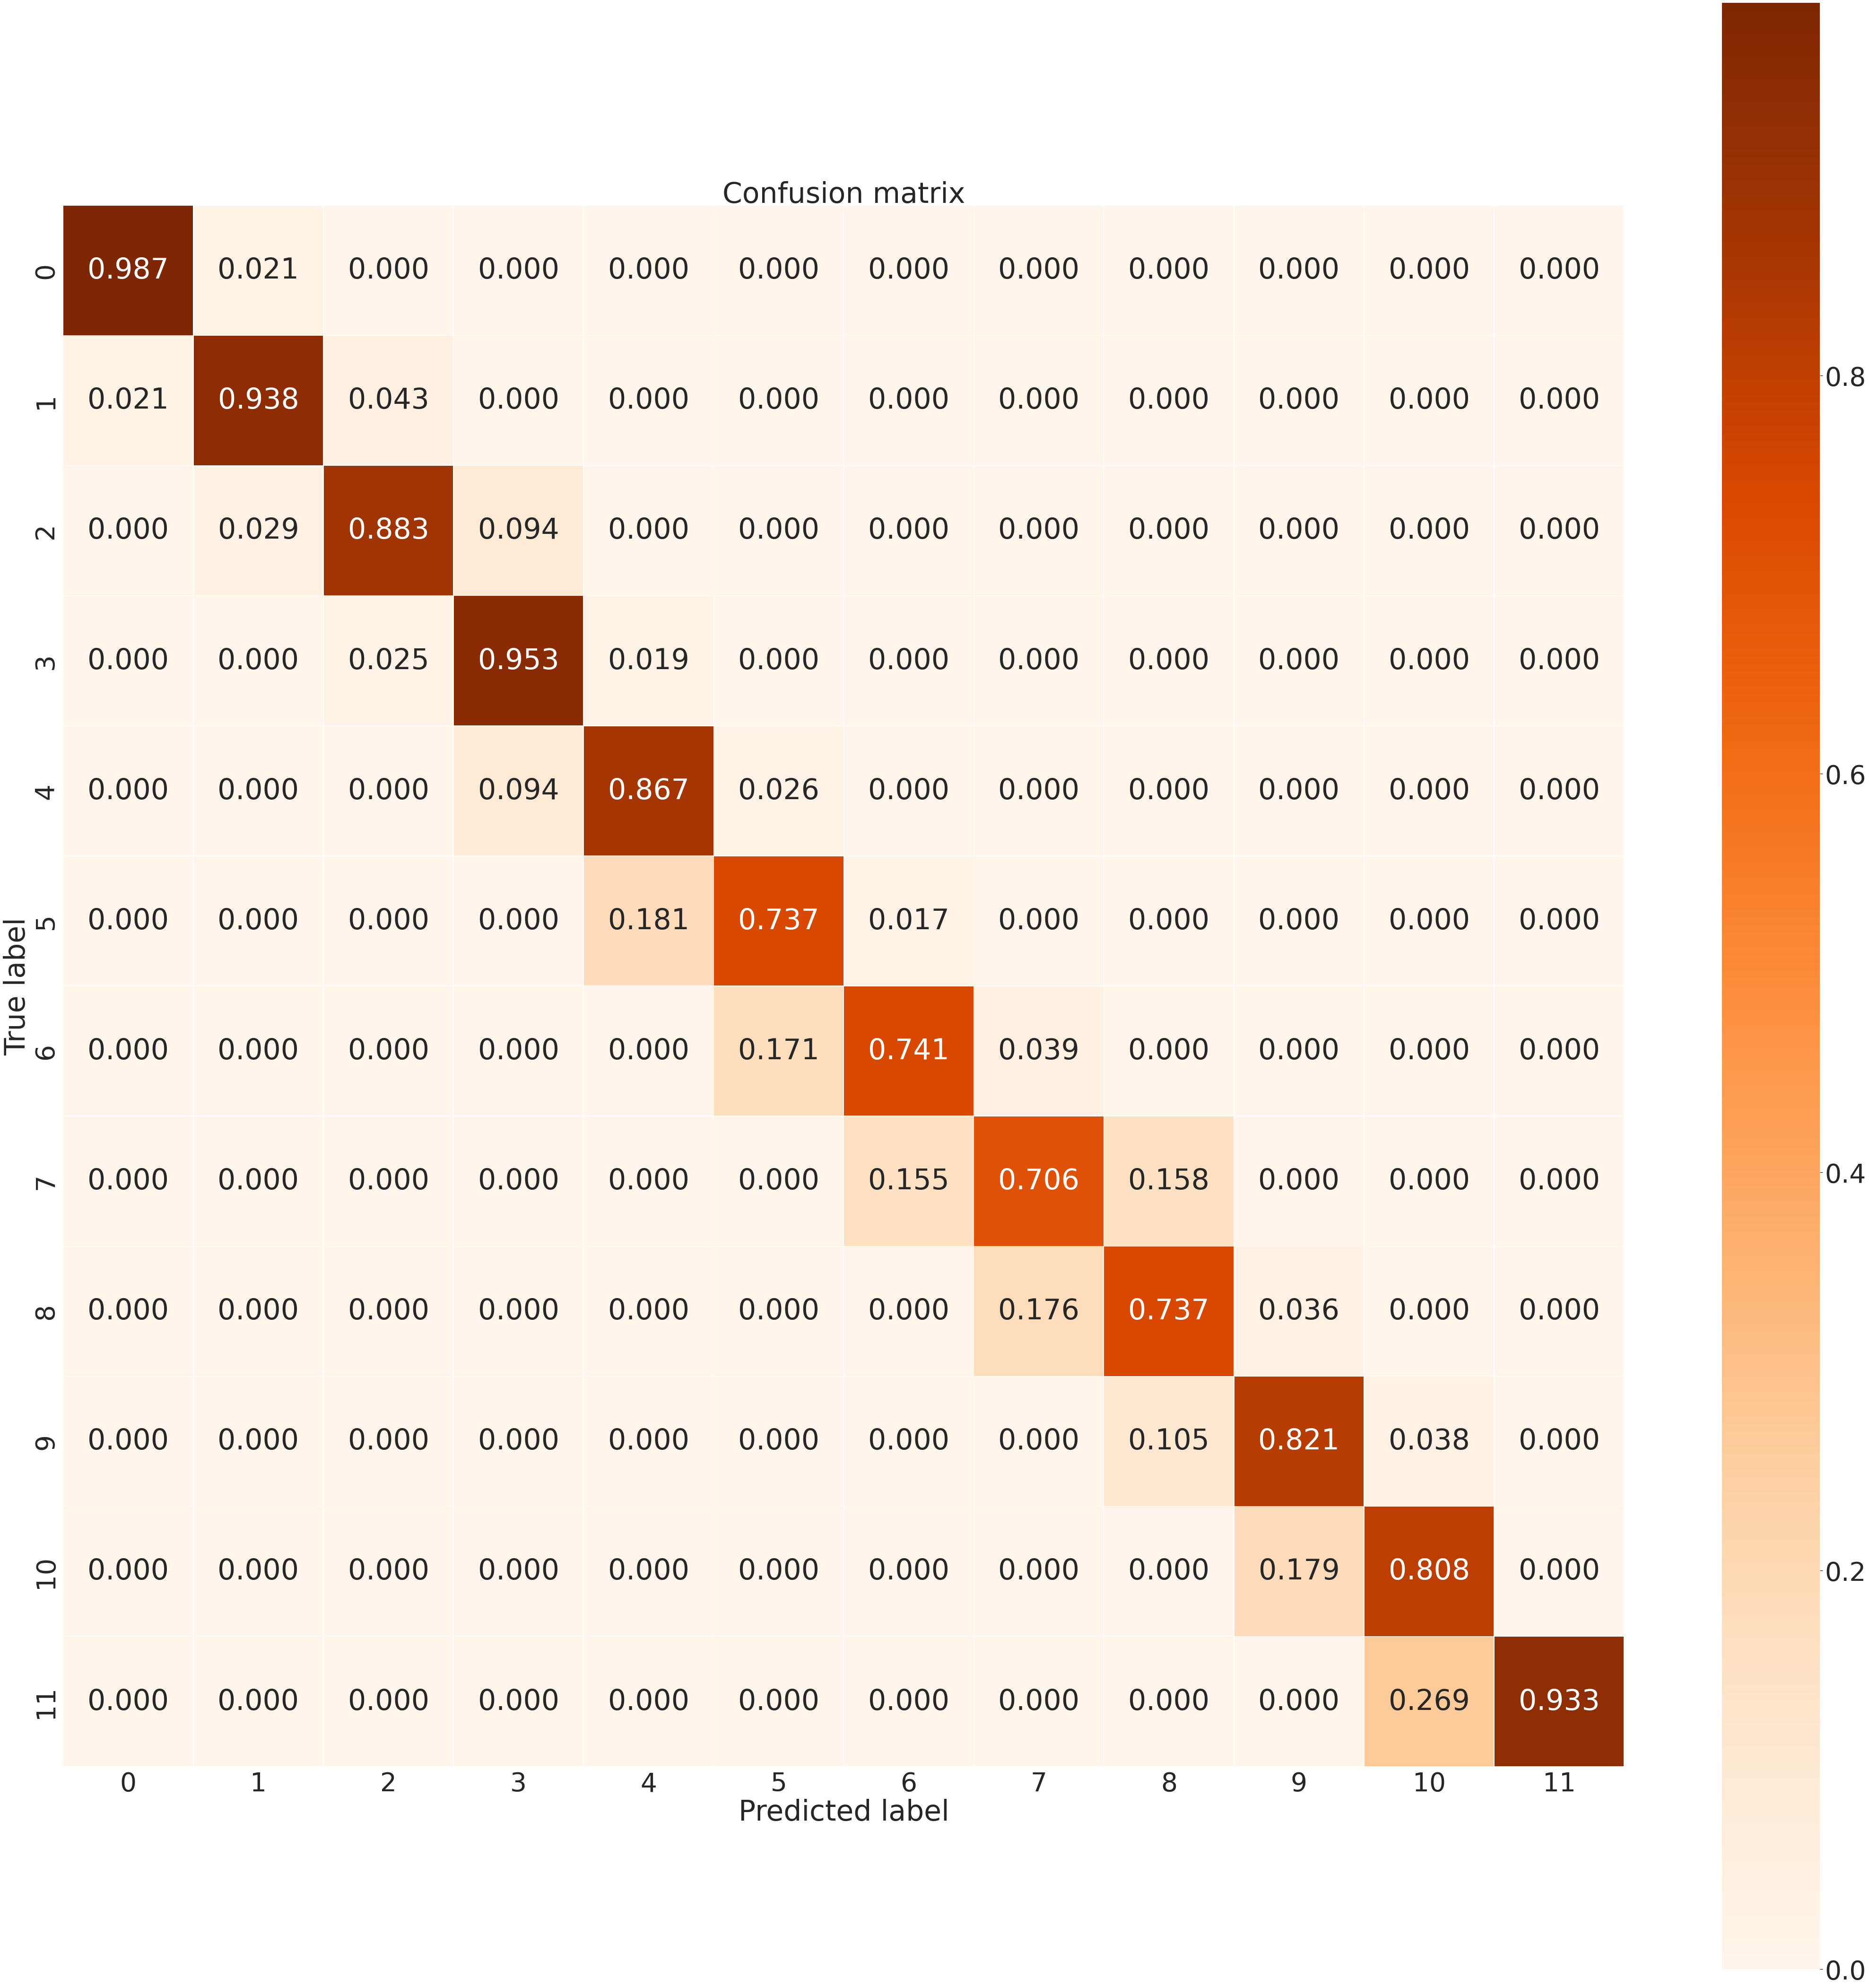
\includegraphics[width=.6\linewidth]{sections/images/section3/confusion_matrix.png}
    \caption{\gls{dnn} Classification - Confusion Matrix}
    \label{fig:confusion_matrix}
\end{figure}
\subsection{Comparison with analytical formula}
It is possible to use the analytical formula in \cref{eq:demagn_formula_approx} to predict the maximum overload. As already discussed, it is a simplified formula, and worse accuracy is excepted.

The same dataset of $7000$ samples has been used, and then the result of the function was rounded with different rounding method. Rounding is needed to make the analytical and \gls{ml} results comparable by the same metrics (accuracy).

The used rounding method are
\begin{itemize}
    \item \emph{Nearest}: rounds the number to the closest integer.
    \item \emph{Ceil}: rounds a number to the closest integer value larger than the current number.
    \item \emph{Floor}: rounds the integer to the closest integer smaller than the current one.
\end{itemize}

The resulting accuracy of the formula with different rounding methods is shown on the following table:
\begin{center}
    \begin{table}[H]
       \renewcommand{\arraystretch}{1.2}
        \centerline{
        \centering
        \begin{tabular}{|c|c|}
        \hline
        Rounding method &Accuracy \\
        \hline
        Nearest & $0.588$ \\
        \hline
        Ceil & $0.240$ \\
        \hline
        Floor  & $0.685$ \\
        \hline
        \end{tabular}}
    \end{table}
\end{center}
The floor rounding got the best accuracy, the analysis will be focusing on it. Confusion matrix of the analytical model using floor rounding can be seen in \cref{fig:confusion_matrix_analytical}. Precision, Recall and f1-score are the following:
\begin{lstlisting}[basicstyle=\ttfamily\footnotesize]
              precision    recall  f1-score   support

           0      0.722     0.901     0.801      1903
           1      0.520     0.454     0.485      1211
           2      0.815     0.608     0.697       812
           3      0.945     0.783     0.857       641
           4      0.911     0.759     0.828       526
           5      0.721     0.692     0.706       380
           6      0.609     0.581     0.595       289
           7      0.413     0.377     0.394       257
           8      0.239     0.277     0.257       191
           9      0.177     0.209     0.191       139
          10      0.261     0.281     0.271       128
          11      0.826     0.937     0.878       523

    accuracy                          0.685      7000
   macro avg      0.597     0.572     0.580      7000
weighted avg      0.692     0.685     0.682      7000
\end{lstlisting}
\begin{figure}[H]
    \centering
    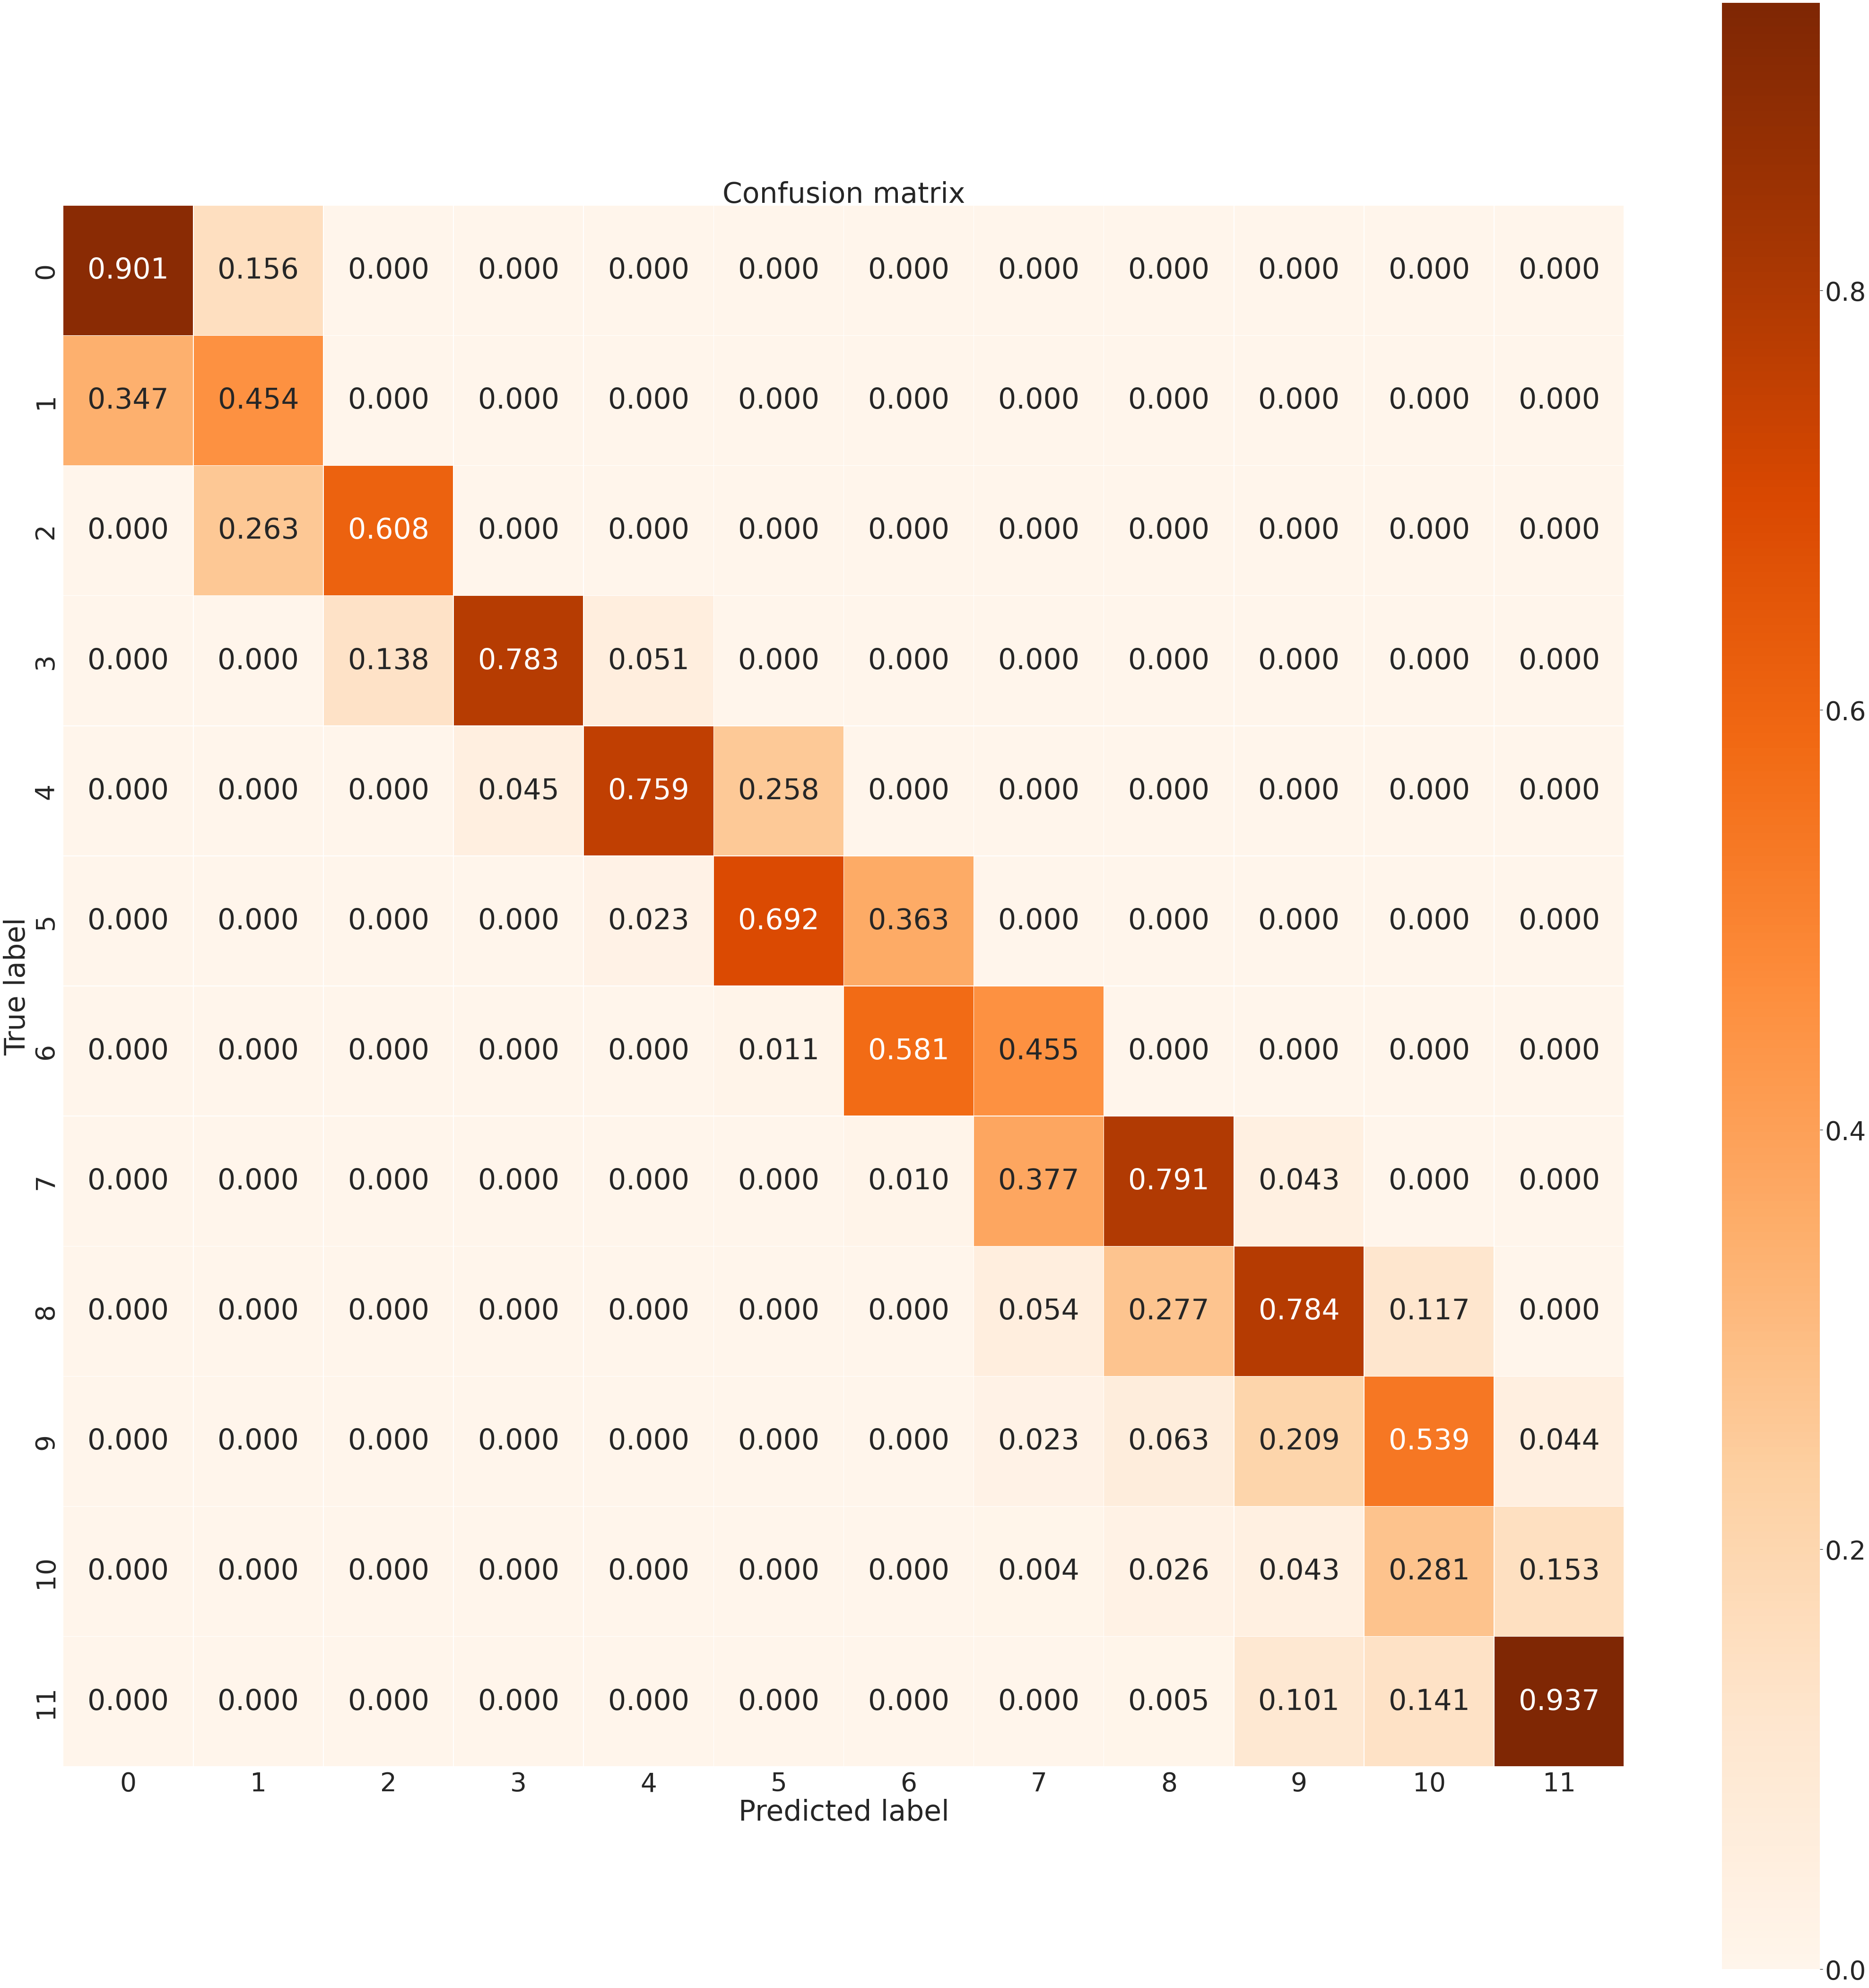
\includegraphics[width=.6\linewidth]{sections/images/section3/confusion_matrix_analytical.png}
    \caption{Analytical Model - Confusion Matrix}
    \label{fig:confusion_matrix_analytical}
\end{figure}
\section{Results, future works and improvements}
In the following table, all the interesting result metrics can be appreciated:
\begin{center}
    \begin{table}[H]
       \renewcommand{\arraystretch}{1.2}
        \centerline{
        \centering
        \begin{tabular}{|l|c|c|}
        \hline
        &Validation loss &Validation accuracy \\
        \hline
        Linear regression - one variable&$0.8425 $ & $0.3482$ \\
        \hline
        Linear regression - multi variable&$0.6756 $ & $0.4089$ \\
        \hline
        NON Linear regression - one variable $L_{magn}$&$0.7681 $ & $0.3518$ \\
        \hline
        NON Linear regression - one variable $B_{mr}$&$1.0235 $ & $0.3357$ \\
        \hline
        NON Linear regression - multi variable &$0.1590 $ & $0.4339$ \\
        \hline
        \gls{dnn} classification model&$0.2841 $ & $0.8893$ \\
        \hline
        Analytical Equation&$--$ & $0.685$ \\
        \hline
        \end{tabular}}
    \end{table}
\end{center}
It can be seen that the \gls{dnn} classification model outperforms any other model used in this report. this work can be considered as a good start for \gls{ml} application in \gls{pmsm} demagnetization.

It is proper to remember that this model is strongly limited: only one type of motor is used, with limited amount motor specifications, and with fixed materials. A future work could be to extend the network, and make it work for more type of motors. Despite this limitation, it is possible to see how \gls{ml} can be successfully be used to speed up and improve electric motor design, that was the initial target of this work.

In \cref{fig:model_dnn}, the final network of the \gls{dnn} classifier.
\begin{figure}[H]
    \centering
    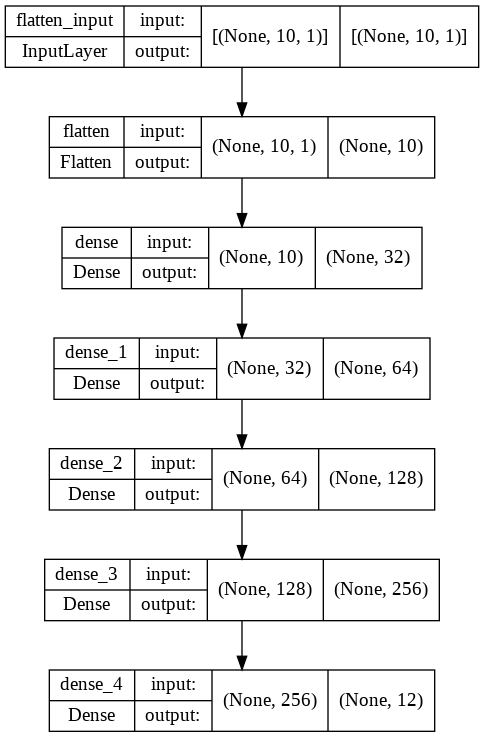
\includegraphics[width=.4\linewidth]{sections/images/section3/network.png}
    \caption{\gls{dnn} Classification network}
    \label{fig:model_dnn}
\end{figure}



\newpage
\printglossary[type=\acronymtype]
\medskip
\bibliographystyle{unsrt}
\bibliography{bibliography}

\begin{appendices}
\newgeometry{
    textheight=740pt,left=20px,right=20px
    %top=3cm,bottom=3cm,right=2cm,left=2.5cm,headheight=14pt
}
\fancyhf{}
\pagestyle{fancy}
\rfoot{Page \thepage}
\section{m400-50a}\label{appendixb}
%\subsection*{IEC.250/6.260 lamination}
\begin{center}
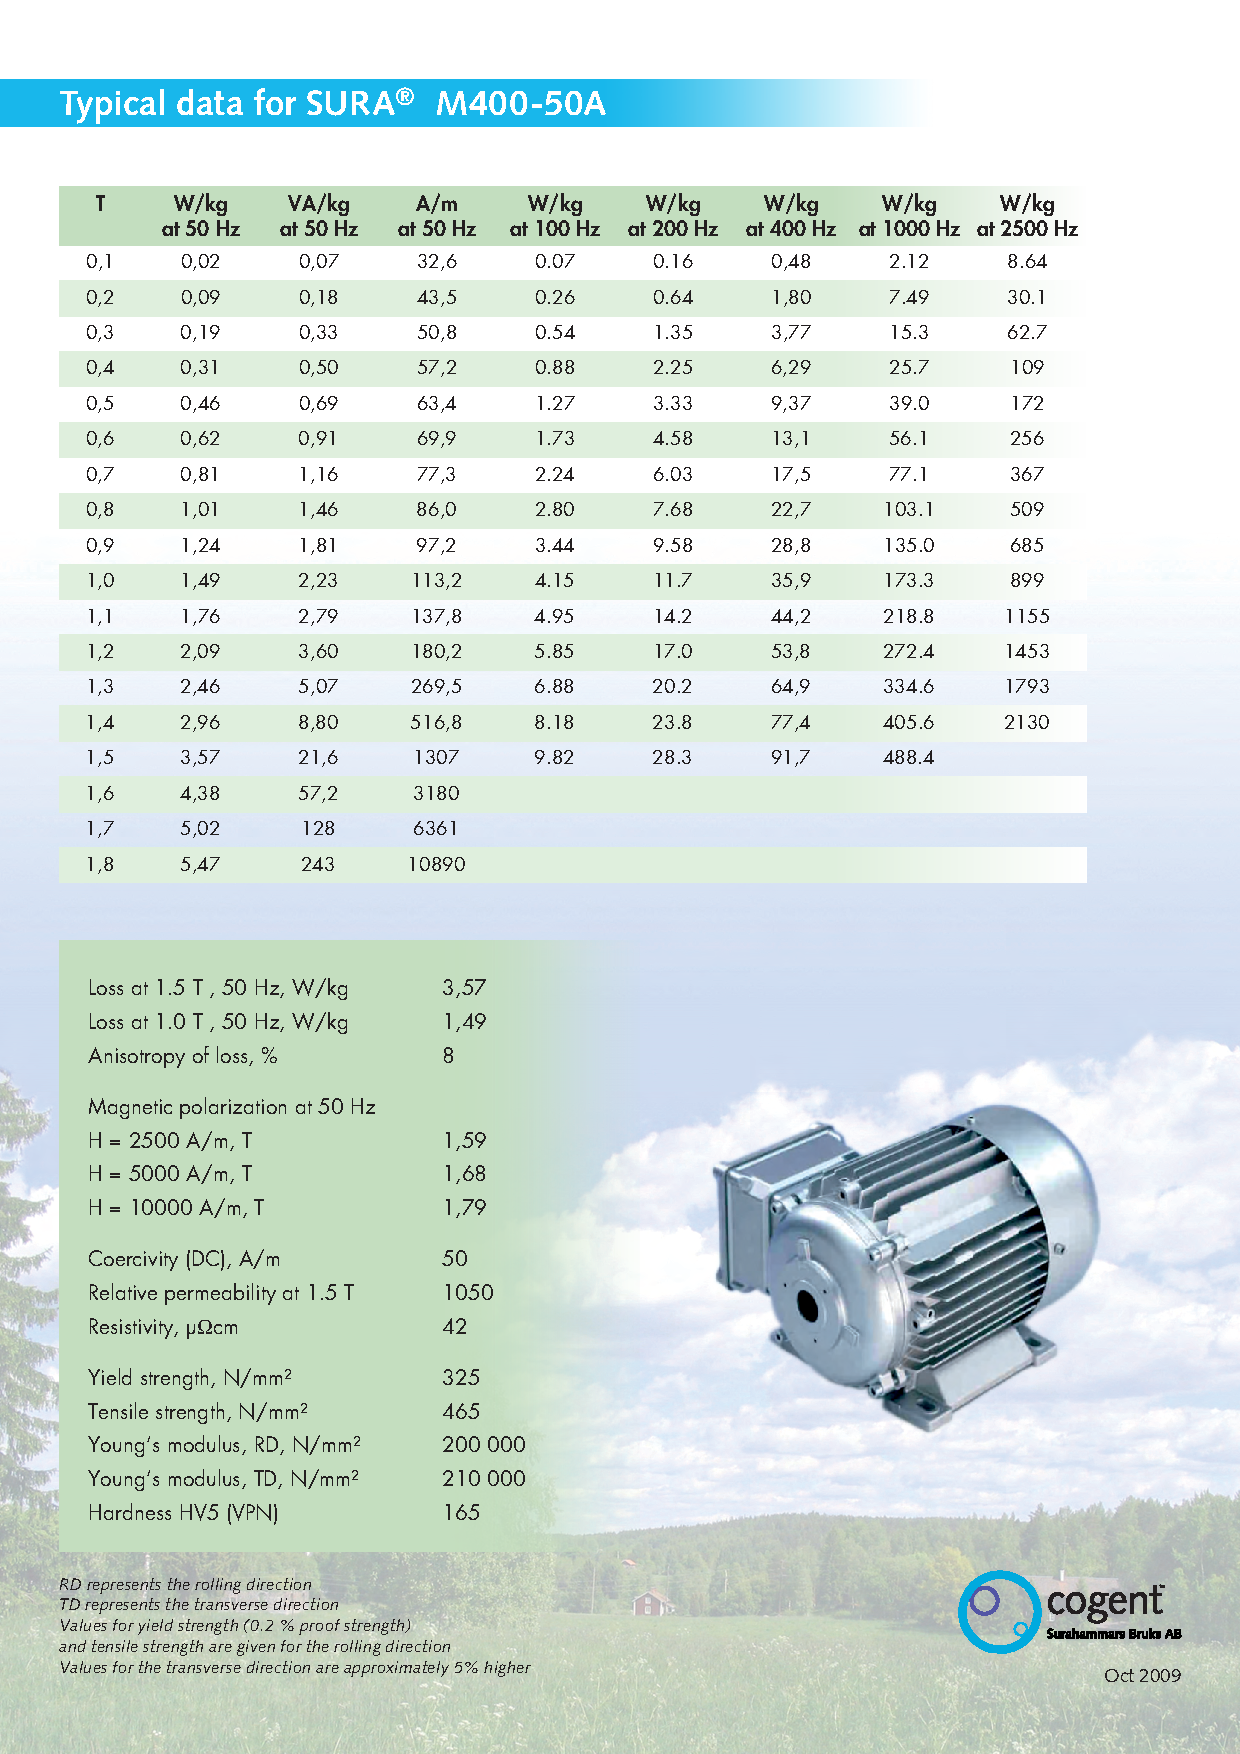
\includegraphics[height=690pt]{extra/m400-50a.pdf}
\end{center}
\section{DAMID 180 copper winding wire}\label{appendixdamid}
\begin{center}
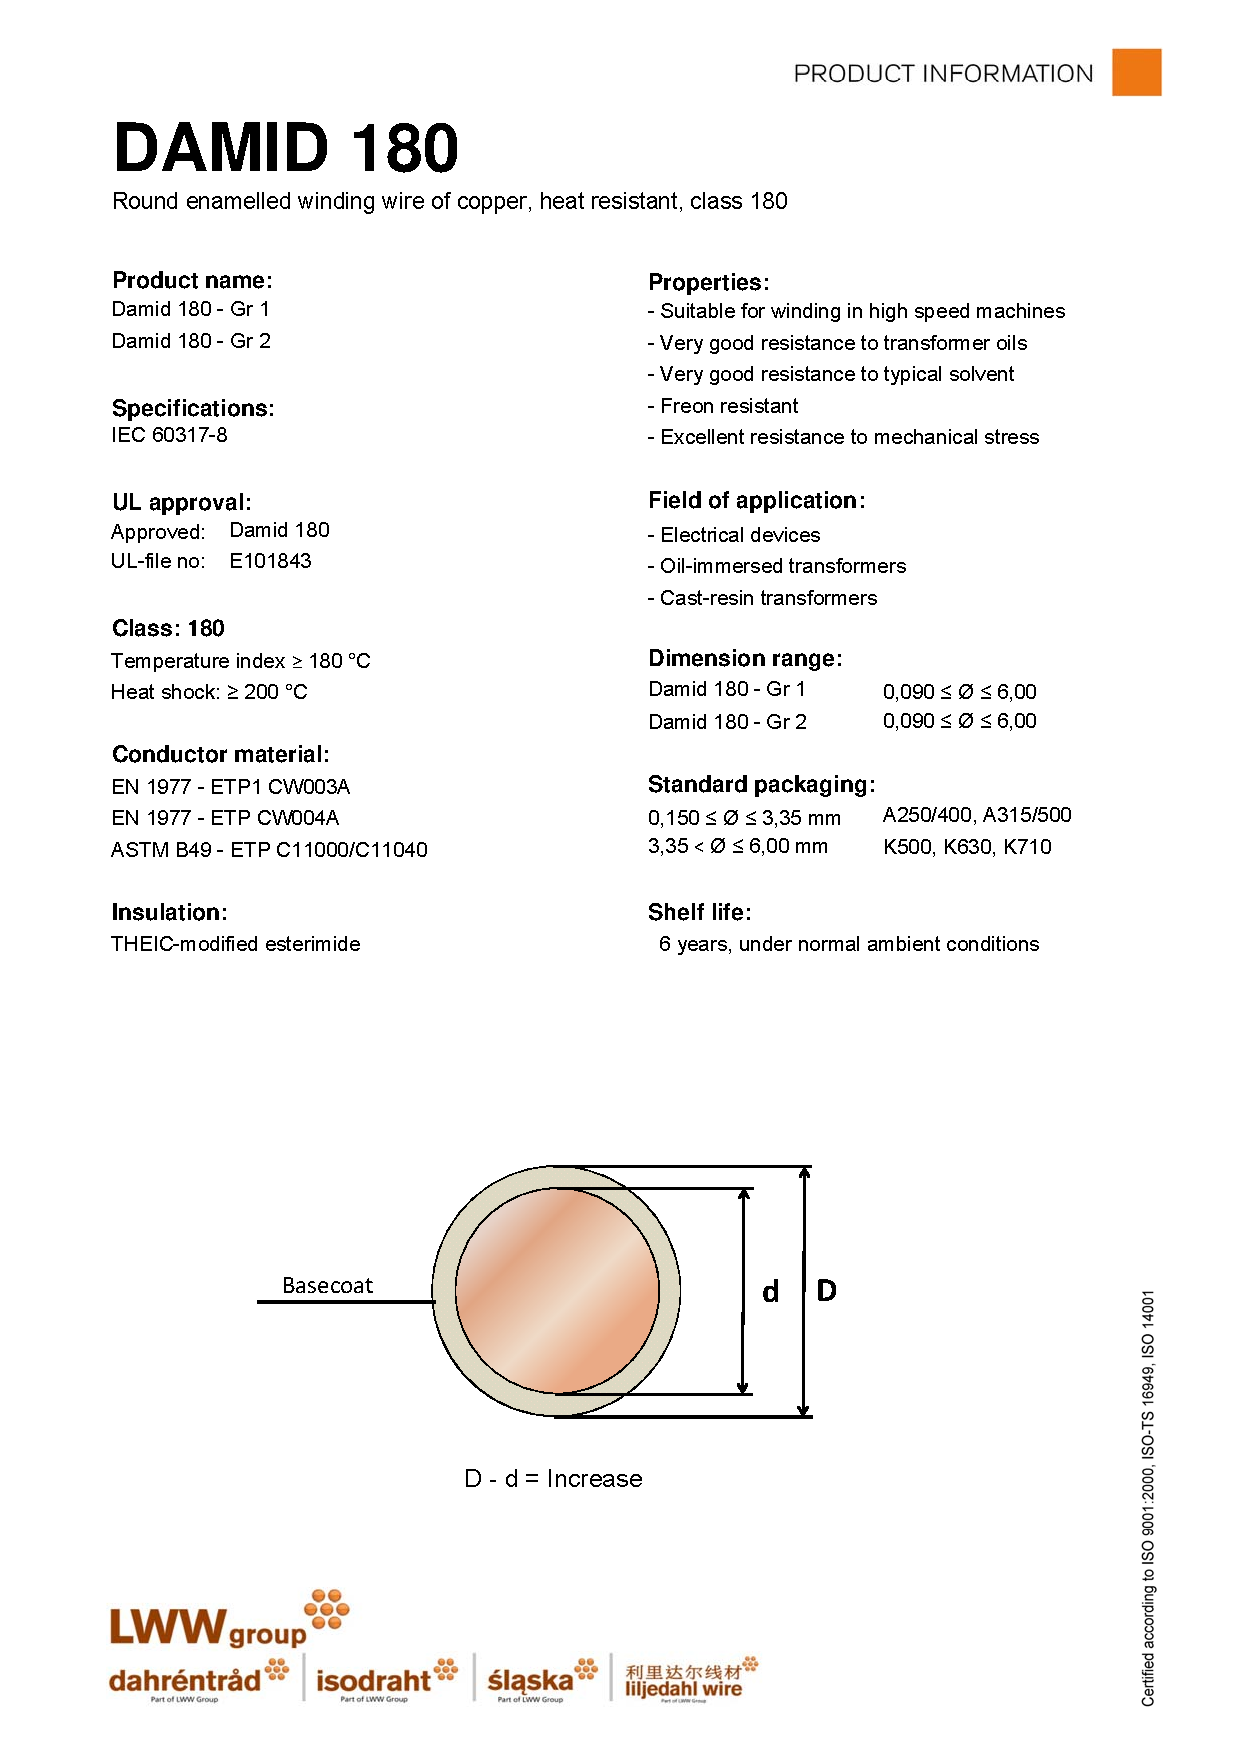
\includegraphics[height=690pt]{extra/DAMID-180.pdf}
\end{center}
\section{Cibas ren35h NeFeb datasheet}\label{appendixmagn}
%\subsection*{IEC.250/6.260 lamination}
\begin{center}
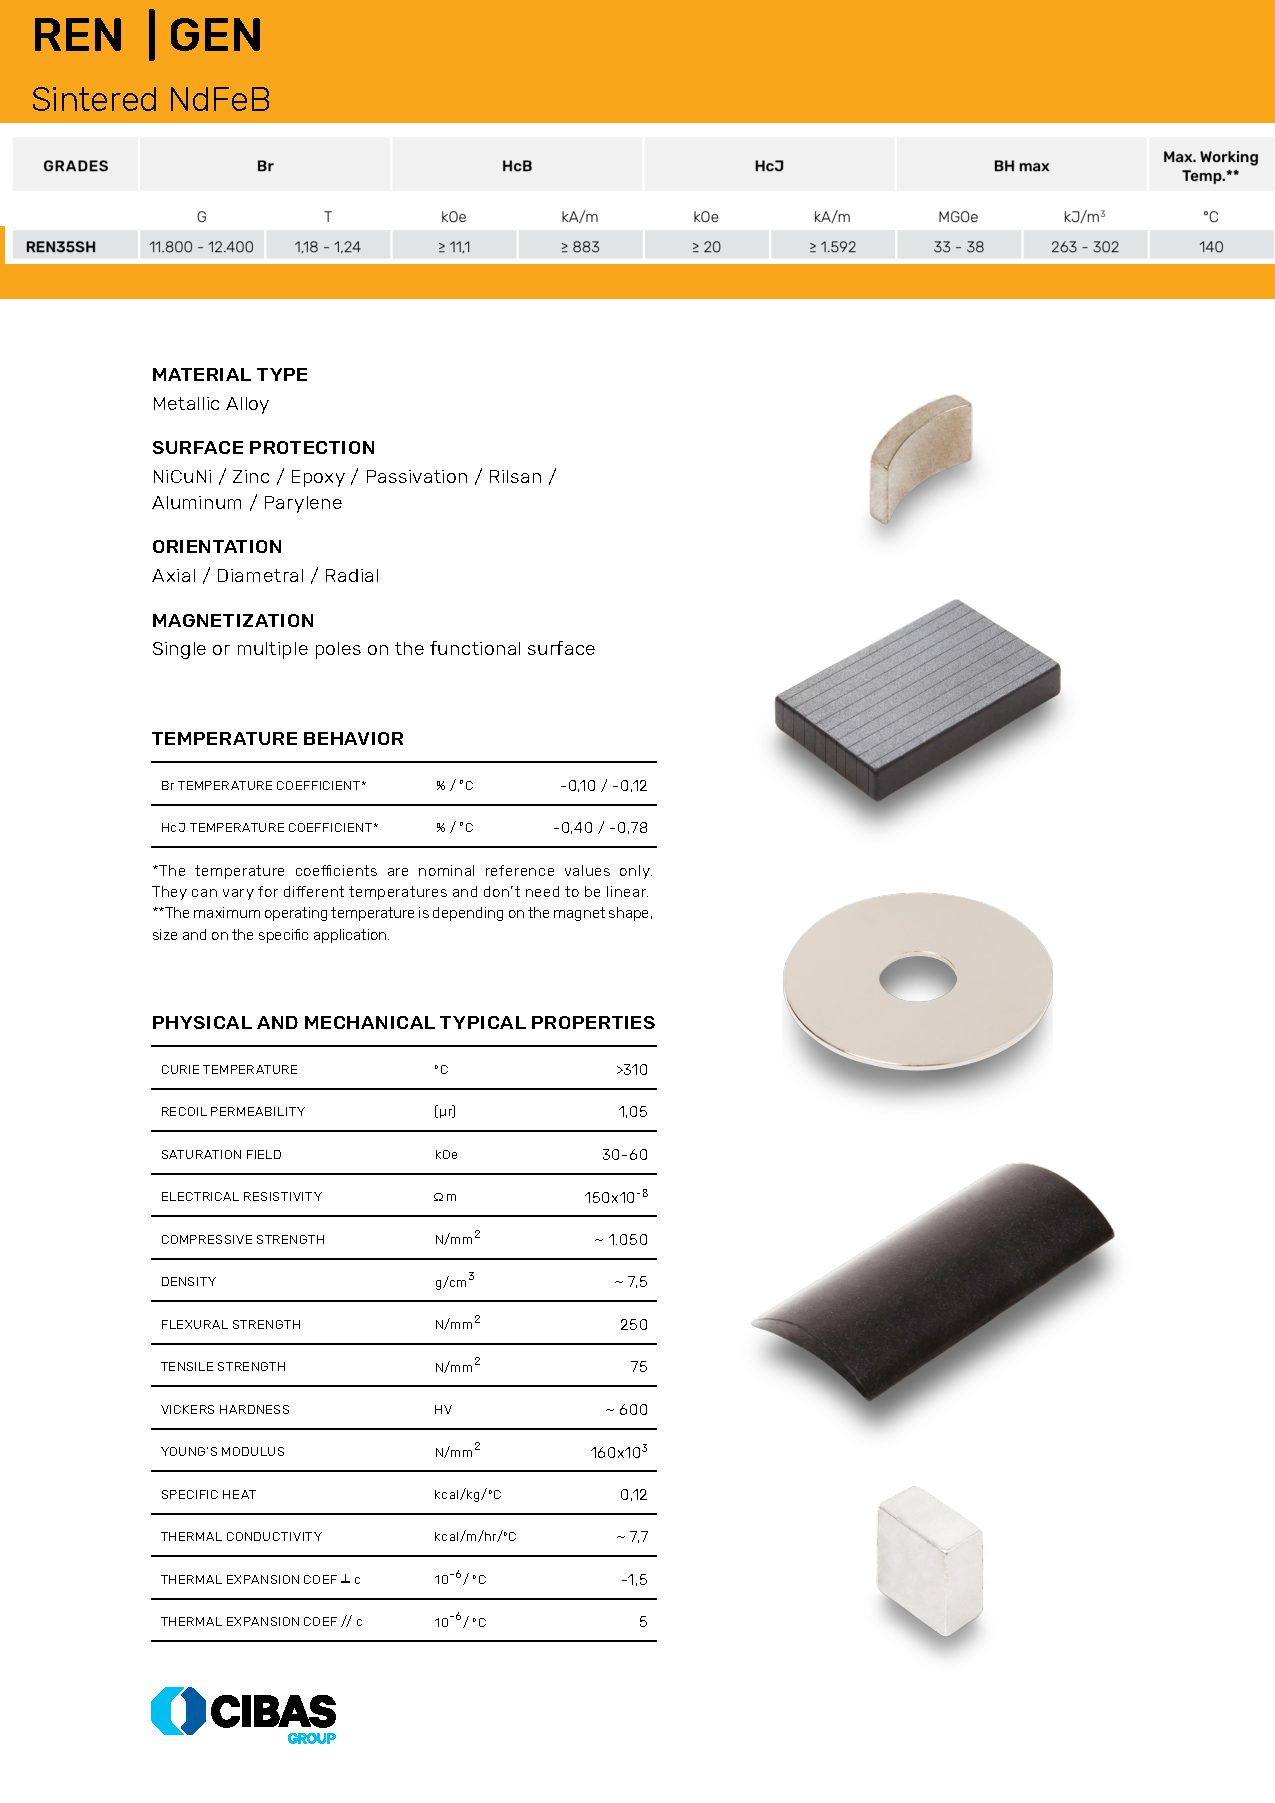
\includegraphics[height=690pt]{extra/cibas_modificato.pdf}
\end{center}


\restoregeometry
\end{appendices}
\end{document}
